%% LyX 2.0.3 created this file.  For more info, see http://www.lyx.org/.
%% Do not edit unless you really know what you are doing.
\documentclass[12pt,english]{article}
\usepackage[latin9]{inputenc}
%\setlength{\headheight}{15pt}
%\usepackage{fancyhdr}
%\pagestyle{p}
\setcounter{secnumdepth}{3}
\setcounter{tocdepth}{3}
\usepackage[T1]{fontenc}
\usepackage{mathtools}
\usepackage{amssymb}
\usepackage{dot2texi}
\usepackage{listings}
\usepackage{tikz}
\usepackage{graphicx}
\usepackage{setspace}
\usepackage{pdfpages}
\onehalfspacing
\usepackage[unicode=false,pdfusetitle,
 bookmarks=true,bookmarksnumbered=true,bookmarksopen=false,
 breaklinks=false,pdfborder={0 0 0},backref=false,colorlinks=false]
 {hyperref}

\newcommand{\Keywords}[1]{\par\noindent
{\small{\em Keywords\/}: #1}}
\usepackage{color}

\definecolor{mygreen}{rgb}{0,0.6,0}
\definecolor{mygray}{rgb}{0.5,0.5,0.5}
\definecolor{mymauve}{rgb}{0.58,0,0.82}
\lstset{
backgroundcolor=\color{white},   % choose the background color; you must add \usepackage{color} or \usepackage{xcolor}
  basicstyle=\footnotesize,        % the size of the fonts that are used for the code
  breakatwhitespace=false,         % sets if automatic breaks should only happen at whitespace
  breaklines=true,                 % sets automatic line breaking
  captionpos=b,                    % sets the caption-position to bottom
  commentstyle=\color{mygreen},    % comment style
  deletekeywords={...},            % if you want to delete keywords from the given language
  escapeinside={\%*}{*)},          % if you want to add LaTeX within your code
  extendedchars=true,              % lets you use non-ASCII characters; for 8-bits encodings only, does not work with UTF-8
  frame=single,                    % adds a frame around the code
  keywordstyle=\color{blue},       % keyword style
  language=C,                      % the language of the code
  morekeywords={*,...},            % if you want to add more keywords to the set
  numbers=left,                    % where to put the line-numbers; possible values are (none, left, right)
  numbersep=5pt,                   % how far the line-numbers are from the code
  numberstyle=\tiny\color{mygray}, % the style that is used for the line-numbers
  rulecolor=\color{black},         % if not set, the frame-color may be changed on line-breaks within not-black text (e.g. comments (green here))
  showspaces=false,                % show spaces everywhere adding particular underscores; it overrides 'showstringspaces'
  showstringspaces=false,          % underline spaces within strings only
  showtabs=false,                  % show tabs within strings adding particular underscores
  stepnumber=1,                    % the step between two line-numbers. If it's 1, each line will be numbered
  stringstyle=\color{mymauve},     % string literal style
  tabsize=2,                       % sets default tabsize to 2 spaces
  title=\lstname                   % show the filename of files included with \lstinputlisting; also try caption instead of title
}

\makeatletter
%%%%%%%%%%%%%%%%%%%%%%%%%%%%%% User specified LaTeX commands.
\usepackage[english]{babel}
\newcommand{\BigO}[1]{\ensuremath{\operatorname{O}\bigl(#1\bigr)}}


\makeatother

\begin{document}

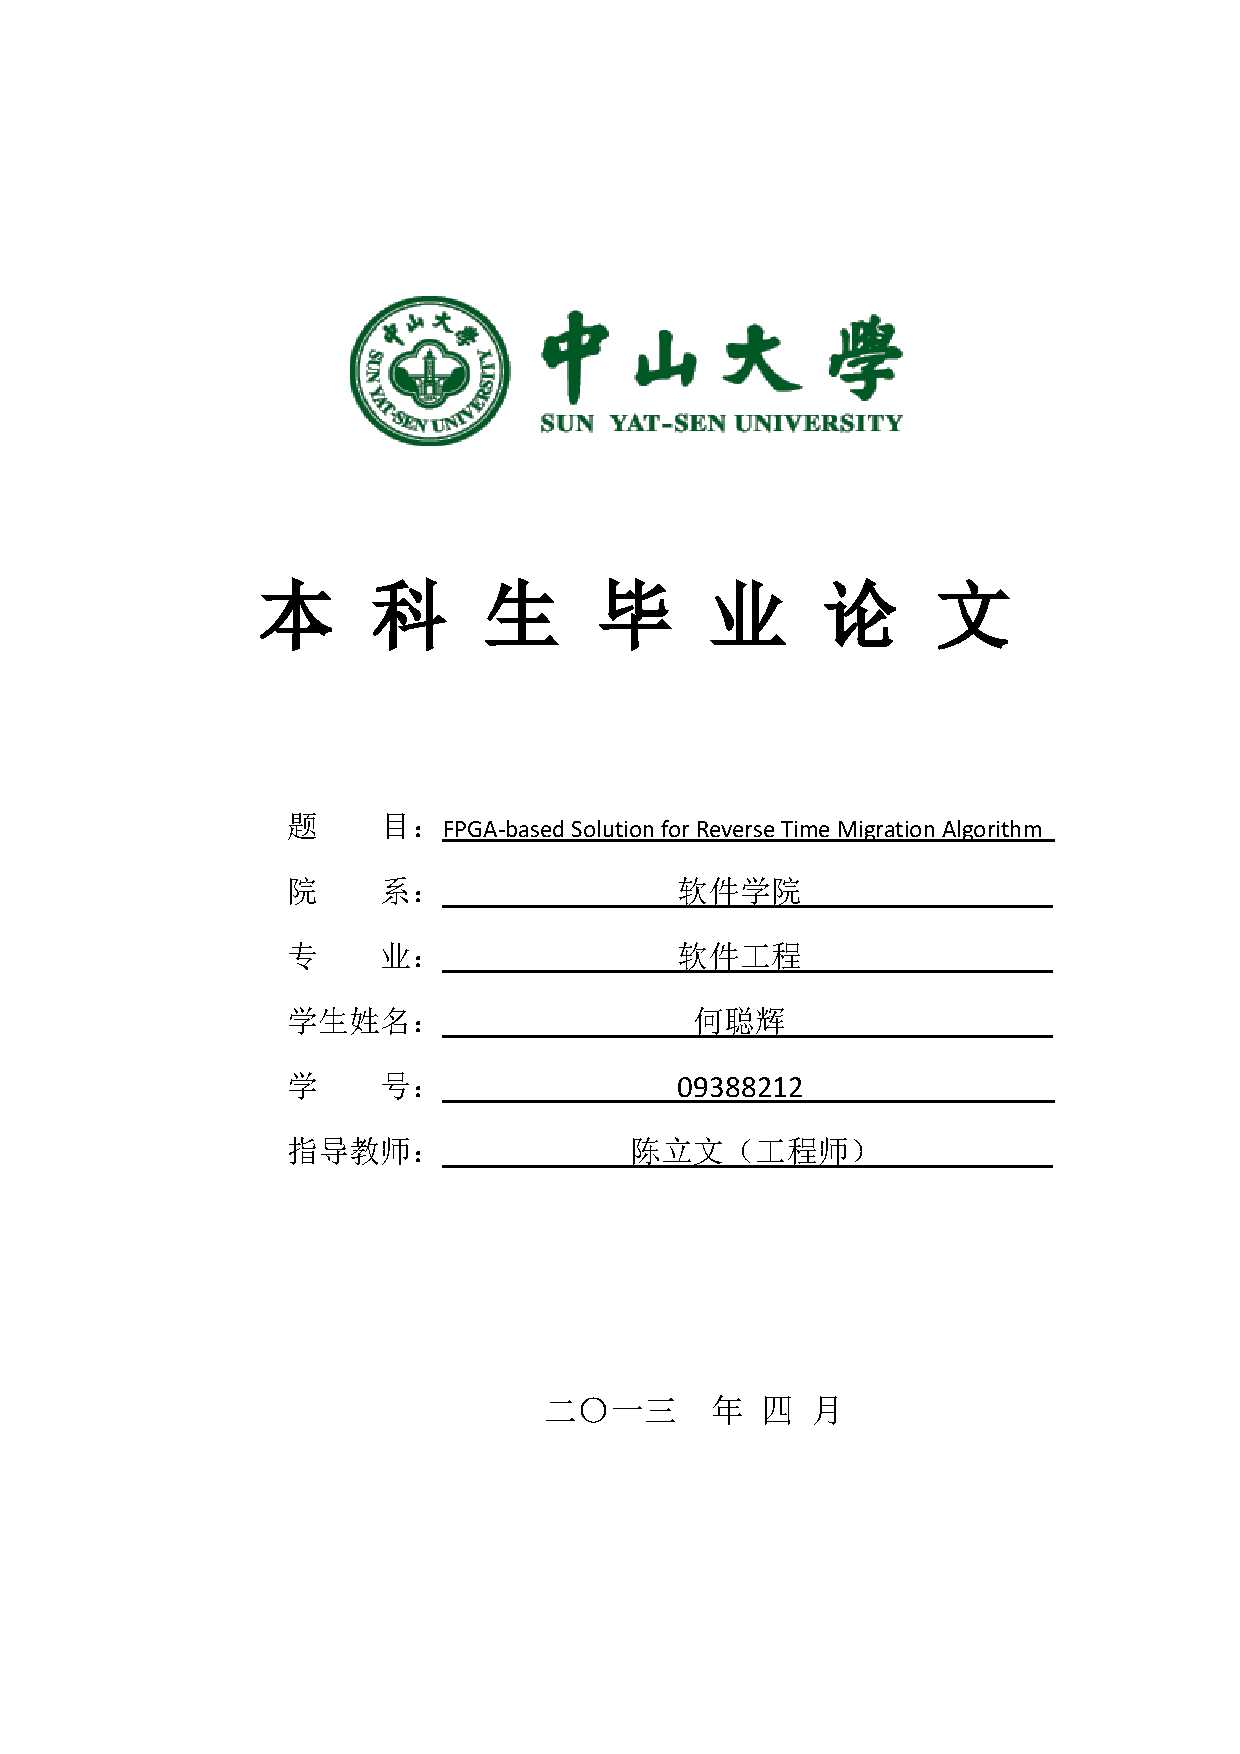
\includepdf{appendix/cover.pdf}

% create an blank page
\newpage
\thispagestyle{empty}
\mbox{}

\begin{abstract}

  The goal of exploration seismology is to find oil and gas reservoirs by
  seismically imaging the earth’s reflectivity distribution The
  conventional one-way wave equation pre-stack depth migration algorithm is
  relatively fast but not able to identify the potential existence of
  hydrocarbon in complex geology. The Reverse time pre-stack depth
  migration (RTM) , which use the two way acoustic wave equation, offers
  insights into complex geology that were previously impossible to
  interpret or understanding using seismic data.  However it is the most
  computationally-demanding algorithm in the oil and gas exploration which
  was considered impractical for production 3D depth imaging project using
  conventional CPUs. Thus hardware accelerator like GPUs and Field
  Programmable Gate Arrays (FPGAs) emerged and have been used as an
  alternative for the conventional computing architectures (CPUs) in
  science computing application and have shown considerable speed-ups.
  Compared with CPUs, FPGA has a better performance but low power
  consumption where logics and algorithms are coded directly into hardware,
  however, only a few applications are implemented on FPGA because the
  steep learning curve for the developers. This thesis, this work, presents
  a solution that takes advantages of FPGA's flexibility to explore
  efficiently data reuse for the 3D Reverse Time Migration algorithm, the
  seismic modeling. Compared with the CPU implementation using two
  quad-core Intel i7 CPUs, the FPGA-based solution without any
  optimization achieves 6x speed-ups on one Xilinx V6-SXT475 FPGA.

  \vspace{4mm}

  \noindent{\emph{Keywords:} \textbf{Reverse Time Migration (RTM); Field
  Programmable Gate Array (FPGA); Stencil; Performance}}
\end{abstract}


\tableofcontents

% vim:ts=4:sw=4
%
% Copyright (c) 2008-2009 solvethis
% Copyright (c) 2010-2012 Casper Ti. Vector
% Public domain.

\specialchap{绪言}

本文档是“北京大学论文文档模版”的说明文档,
同时也是使用模版的一个示例。

pkuthss 文档模版由三部分构成:
\begin{itemize}
	\item \textbf{pkuthss 文档类}:
		其中进行了学位论文所需要的一些基本的设定,
		主要包括对基本排版格式的设定和提供设置论文信息的命令。
	\item \textbf{pkuthss-extra 宏包}:
		其中实现了学位论文中用户可能较多用到的一些额外功能,
		例如自动在目录中加入参考文献和索引的条目和%
		自动根据用户设定的文档信息对所生成 pdf 的作者、标题等属性进行设置等。
	\item \textbf{说明(示例)文档}:
		说明文档即本文档,
		在安装(见第 \ref{sec:inst} 节)之后应该可以用 \TeX{} 系统提供的
		\verb|texdoc| 命令调出:
\begin{Verbatim}[frame=single]
texdoc pkuthss
\end{Verbatim}
		同时,
		本文档的源代码(位和本文档的 pdf 文件处于同一目录下)%
		也正是用户撰写自己的学位论文时的一个模版:
		用户只需按照模版中的框架修改代码,
		即可写出自己的论文。
\end{itemize}

在此之前,包括 dypang\supercite{dypang}、FerretL\supercite{FerretL}、%
lwolf\supercite{lwolf}、Langpku\supercite{Langpku}、%
solvethis\supercite{solvethis} 等的数位网友均做过学位论文模版的工作。
本论文模版是 solvethis 的 pkuthss 模版的更新版本,
更新的重点是重构和对新文档类、宏包的支持。

pkuthss 文档模版现在的维护者是 Casper Ti. Vector\footnote%
{\href{mailto:CasperVector@gmail.com}{\texttt{CasperVector@gmail.com}}}。%
pkuthss 文档模版目前托管在 Google Code 上,
其项目主页是:\\
\hspace*{\parindent}\url{http://code.google.com/p/caspervector/}


\section{Field Programmable Gate Array}

\subsection{An Overview of FPGA}
Field Programmable Gate Array (FPGA) is a type of integrated circuit (IC)
containing a matrix of logic cells that can be programmed by a user to act
as an arbitrary integrated circuit.

The first field programmable gate array is manufactured by Xilinx
in 1985. However, compared with the widespread of computers, FPGA
was primarily made use of in telecommunications and networking in
the 1990s due to both the sophistication and the volume of the production.

Using the pre-built logic blocks and
programmable routing resources, you can configure these chips to implement
custom hardware functionality in high performance. For example, one can implement a
interrupt controller, a digital filter or even a processor on the basic of
FPGA.

In the past, FPGA technology could be used only by
engineers with a deep understanding of digital hardware design. Thus FPGA is
not as widely use as general purpose processor around the world. But in
the recent years, some companies encapsulated the underlining details of
FPGA and rised several suits of development tools kits to provide a higher
abstract interface for develops. The developers who designing the FPGA now
just need to task in the software and compile them down to a configuration
file or bitstream that contains information on how to components should be
wired together, which makes the task much easier and more and more
developers devotes their energies to FPGA.

\subsection{The Architecture of FPGA}

A typical layout of FPGA (see Figure~\ref{fig:fpga_arch}) is an array of
interconnected programmable logic blocks or configurable logic blocks. It
provides the designer with programmable logic blocks that contain the pool
of combinatorial blocks and flip-flops to be used in the design. Logic is
often used in conjunction with memory. Clock conditioning has also become
commonplace, and support in the form of Delay Locked Loops (DLLs). Phase
Locked Loops (PLLs) is also provided inside the same silicon chip. Finally,
an FPGA chip does not lead a solitary life isolated from the rest of the
world. It needs to be easily interfaced to other chips or external signals.
In order to make this interfacing easier, FPGA vendors have invested a
great deal of effort in enhancing the flexibility of the input/output
blocks behind the chip pads. Each pad can serve as an input, an output, or
both. The list of electrical standards supported is extensive, and novel
techniques for maximizing bandwidth, such as clocking data in using both
edges of the clock, are widely supported~\cite{fpgaintro}.

\begin{figure}
  \centering
  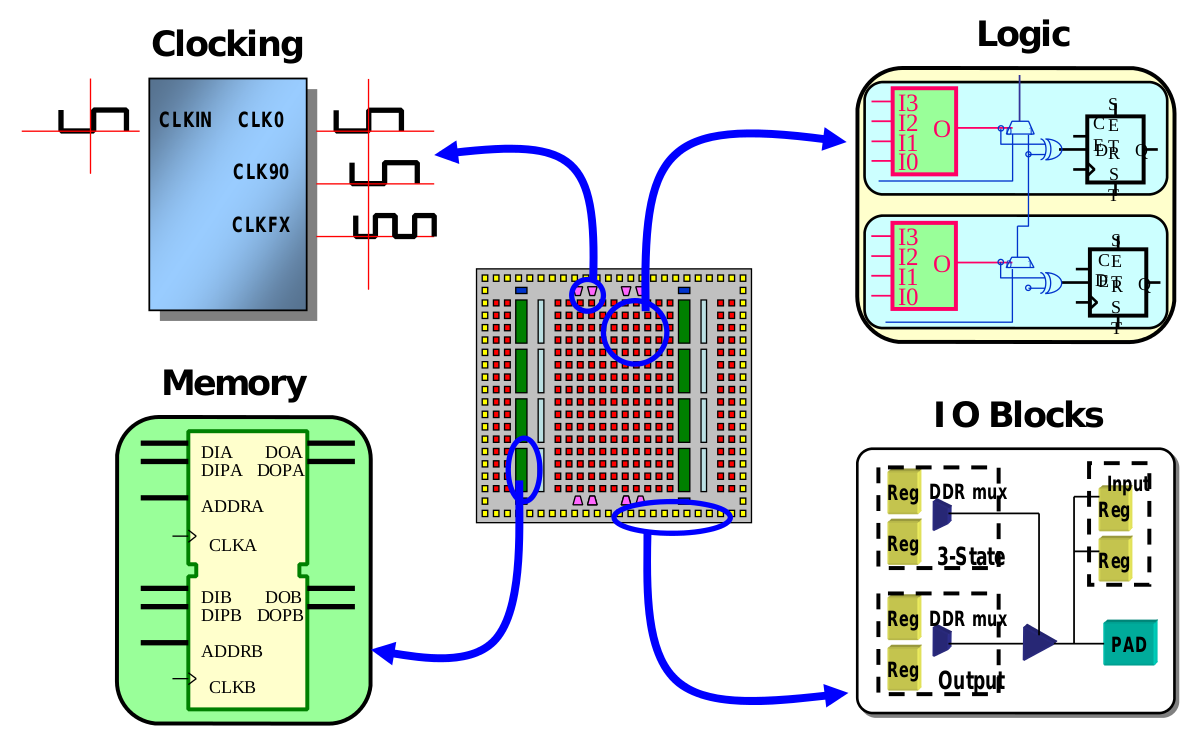
\includegraphics[scale=0.25]{img/fpga_arch.png}
  \caption{Typical structure of modern FPGA}
  \label{fig:fpga_arch}
\end{figure}

Xilinx is the largest vendors of modern FPGA , their latest product, such
as Spartan-3 generation, general consist of five fundamental programmable
functional elements, configurable Logic Blocks (CLBs), Input/Output Blocks
(IOBs), BLOCK RAM, Multiplier Blocks, and Digital Clock Manager (DCM).

\begin{itemize}

  \item \emph{Configurable Logic Blocks (CLBs)} contain flexible Look-Up
    Tables (LUTs) that implement logic plus storage elements used as
    flip-flops or latches. CLBs perform a wide variety of logical functions
    as well as store data.

  \item \emph{Input/Output Blocks (IOBs)} control the flow of data between
    the I/O
    pins and the internal logic of the device. IOBs support bidirectional
    data flow plus 3-state operation. Supports a variety of signal
    standards, including several high-performance differential standards.
    Double Data-Rate (DDR) registers are included.

  \item \emph{Block RAM} provides data storage in the form of 18-Kbit
    dual-port
    blocks.

  \item \emph{Multiplier Blocks} accept two 18-bit binary numbers as inputs
    and
    calculate the product. The Spartan-3A DSP platform includes special DSP
    multiply-accumulate blocks.

  \item \emph{Digital Clock Manager (DCM)} Blocks provide self-calibrating,
    fully
    digital solutions for distributing, delaying, multiplying, dividing,
    and phase-shifting clock signals.
\end{itemize}

These elements are organized as shown in Figure~\ref{fig:spartan_arch},
using the Spartan-3A FPGA
array as an example. A dual ring of staggered IOBs surrounds a regular
array of CLBs in the Spartan-3 and Extended Spartan-3A family. The
Spartan-3E family has a single ring of inline IOBs. Each block RAM column
consists of several 18-Kbit RAM blocks. Each block RAM is associated with a
dedicated multiplier. The DCMs are positioned with two at the top and two
at the bottom of the device, plus additional DCMs on the sides for the
larger devices.

\begin{figure}[h]
  \centering
  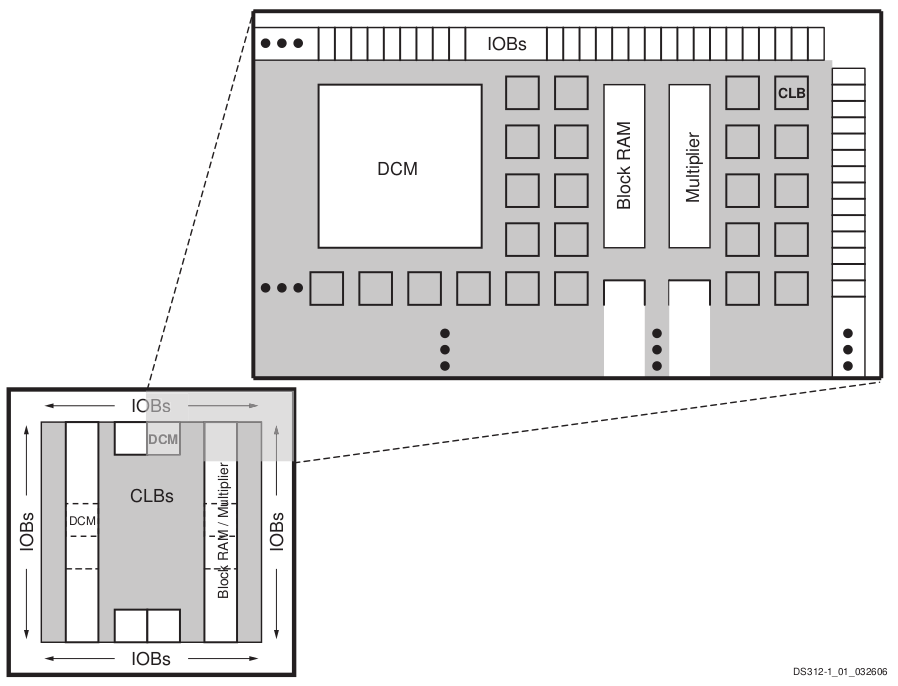
\includegraphics[scale=0.3]{img/spartan_arch.png}
  \caption{Spartan-3A Platform Architecture}
  \label{fig:spartan_arch}
\end{figure}

The Spartan-3 generation features a rich network of traces that
interconnect all five functional elements, transmitting signals among them.
Each functional element has an associated switch matrix that permits
multiple connections to the routing\cite{fpgaug}.

\subsection{Designing FPGA with Maxcompiler}

The usual way to design FPGAs is to write a behavioral model in
a Hardware Description Language (HDL), like Verilog or VHDL, which
supports concurrency and synchronous circuits. Concurrency allows
you to create fully parallel, independent processes, each describing
how to update some variables continuously. Synchronous circuits, instead,
are those made of flip-flops that change their state only on the edge
of some clock signal.

After the design has been written and verified with an HDL simulator,
a compiler creates a list of all the logic gates and the wires (nets)
that must connect them to reproduce the functionality of the HDL model.
After this logic synthesis, layout programs read the netlist and several
constraints files to find out which logic gates inside the FPGAs must
be used and which physical, internal wires must connect them to each
other. The end result is the bit file that the FPGA reads at power-up.

The above kind of FPGA configuring developing is still an obstruct for
those who seldom care much about hardware or digital circuit. In order to
make full use of FPGA, Maxeler Inc, develops a compiler where software
engineer can perform configuring developing with their daily used
developing language, such as C, and Java.

\subsubsection{Maxeler Acceleration Technology}

\emph{Maxcompiler} is a commercial product that is manufactured by Maxeler.
It is a compiler system for Maxeler hardware acceleration solutions using
FPGAs. The compiler system is a good assistant for software engineering
developer to create FPGA configuring because it has a higher abstract of
the underlining subtle hardware information, and then provide a set of
Application Interface for developers.

Figure~\ref{fig:maxeler_acceleration_system} have a sketch of Maxeler
acceleration system architecture. The system comprises several FPGAs
attached directly to the local memory and to a host CPU via PCI Express.

\begin{figure}
  \centering
  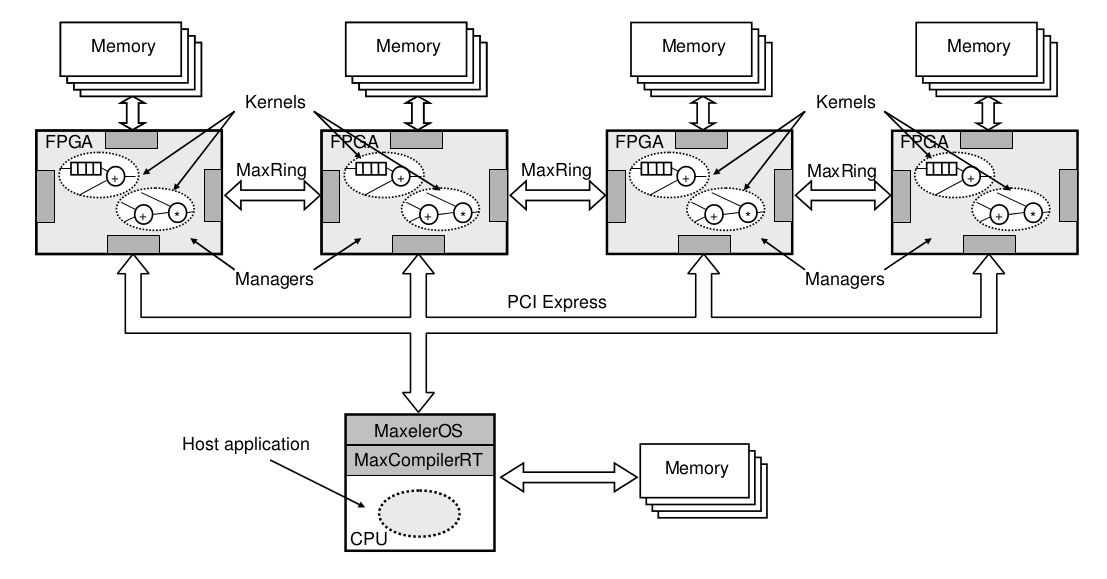
\includegraphics[scale=0.35]{img/overview_of_maxeler_acceleration_system.png}
  \caption{An overview of Maxeler acceleration system}
  \label{fig:maxeler_acceleration_system}
\end{figure}

While developing the application, develops identify the runtime intensive part
and tunning them into FPGA configuration, which is called \emph{kernel} and
\emph{manager} in the acceleration system. After all the configured FPGA
files are compiled and downloaded into FPGA EEPROM, the host (CPU) code
communicate with FPGA with the help of \emph{Maxeler OS}. The Maxeler OS
provide a set of API called \emph{MaxCompierRT}, a runtime library to load
the configuration to FPGA and transfer data from/to FPGA.

The programming paradigm of FPGA designing is different from the general
programming paradigm, such as C/C++. The FPGA gains it high efficiency from
the parallel working of the different Configurable Logic Block (CLB). The
program describes the computations structurally (in space) rather than
specifying the sequence of processor instructions (in
time)\cite{max_white_paper}.

\subsubsection{Development Flow}
If the developer want to accelerate an application after he identifies the
runtime intensive part of the program, what he needs includes three parts,
designing the kernel, manager configuration and adapt the host application.
All the three parts can be easily implemented with the help of Maxeler
compiler tools. Figure \ref{fig:development_flow} presents the development flow with the main
components of MaxCompiler.

\begin{figure}[h]
  \centering
  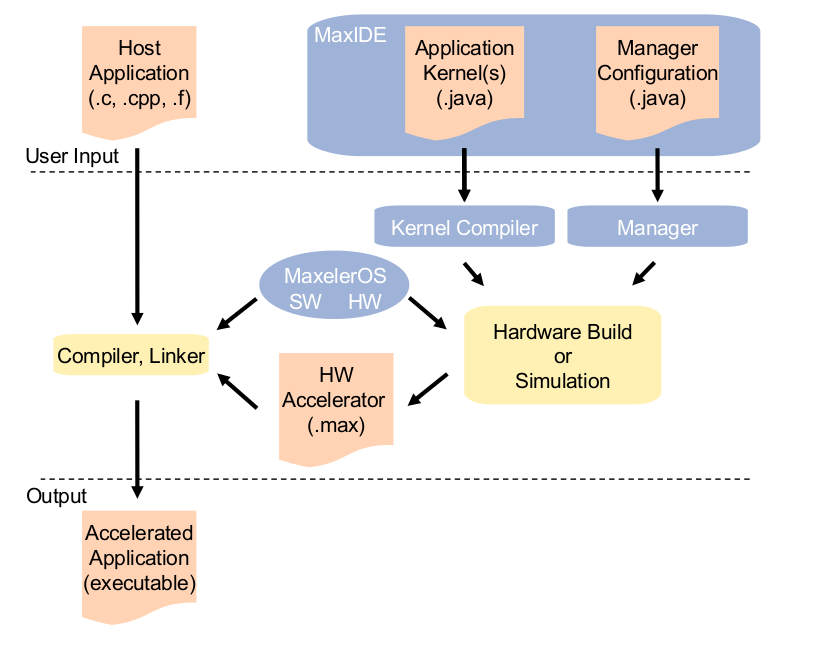
\includegraphics[scale=0.4]{img/development_flow.png}
  \caption{Maxeler development flow}
  \label{fig:development_flow}
\end{figure}

The first stage, designing the kernel, is the most critical part of the
acceleration. Kernel has the similar meaning with that in CUDA GPU
programming, which refers to the most computationally-demanding part that
should be executed in the FPGA/GPU board. Java, the well-known high level
language is used to develop the kernel. Here we just the syntax of Java,
excluding the massive Java library. In addition, the Maxeler provides a set
of library that use to configure the kernel with the help of the
MaxCompiler. Instead of using the phase ``programming to configure kernel
with Java'', it is more appropriate to say ``designing the configure kernel
with Java'', because paradigm of designing the FPGA application with
MaxCompiler is to describe the structure of the logic, rather than telling
the FPGA the sequence of the process instructions, which we use in the
general purpose programming.

When the kernel is well configured, we need to set up a manager for it. The
manager is responsible for how to set up the kernel, for example, pass the
parameter to kernel that kernel expects. What's more, the manager is also
responsible to cooperate the kernels together if there are multiple
kernels, or multiple FPGA boards working for the same problem. The manager
can configure the kernel for simulation or for real work kernel.
Configuring the kernel for simulation is preferred because it saves time to
generate it. A full hardware build may take you hours or even weeks
depending on the complexity of the kernel.

Whenever the simulation kernel or the hardware kernel is build, it is
possible to linked it with the host application. Maxeler provides a set of
runtime library in C/C++ and Fortran to help the programmer to develop. The
communication between the local machine and FPGA device is via the runtime
library and interface, which could help the developer to transform data
from/to the FPGA Device.

The MaxCompiler can link them together in the last stage of the compilation
and generate the ordinary binary executable file.

\subsection{Advantage of FPGA Designing}

FPGA chip adoption across all industries is driven by the fact that FPGAs
combine the best parts of ASICs and processor-based systems. FPGAs provide
hardware-timed speed and reliability, but they do not require high volumes
to justify the large upfront expense of custom ASIC design. Reprogrammable
silicon also has the same flexibility of software running on a
processor-based system, but it is not limited by the number of processing
cores available.

Unlike processors, FPGAs are truly parallel in nature, so
different processing operations do not have to compete for the same
resources. Each independent processing task is assigned to a dedicated
section of the chip, and can function autonomously without any influence
from other logic blocks. As a result, the performance of one part of the
application is not affected when you add more processing.

In addition, FPGAs are blurring the lines between hardware and software in systems.
FPGA devices are inherently soft-programmable and may be changed
dynamically during the operation of a system. More compellingly, FPGA devices
now also contain embedded microprocessors within the logic fabric,
and these microprocessors can run Linux. Imagine a Linux computer
with up to millions of gates of flexible logic immediately around
it. One way to grok this new paradigm is to think of the following:
Software is configuration bits for hardware.

\chapter{Reverse Time Migration Algorithm}

The purpose of the \emph{seismic exploration} is to understand the
constitution of the interior earth as much as possible. As we know, it is
impractical or even impossible to penetrate the earth and put your camera
there to capture the image, other indirect approaches are used to attain
the similar or same result. These approaches includes seismological
measurement, electromagnetic measurement and gravity measurement. As these
approaches are indirect, they usually give a analyze or indication of the
measured result. Some tools, such as computers, are required as part of the
analyze and the capability of the tools may be the bottleneck of the
analyze. For example, in the past, with the poor computational performance
of the computer, the data in only a small region and in a low resolution
could the seismologists analyzed due to the limited computing power.

As the Moore's Law indicates that the number of transistors double every 18
months, the computer gains much more computing power than before. Some
seismological method, which are computationally-demanding, seems not
practical in the past, can be implemented by utilizing the advanced
technology today. One of the most useful but computationally-demanding
algorithm, Reverse Time Migration algorithm, also comes into reality.

Reverse Time Migration is an algorithm of seismic migration. And seismic
migration is one of the most important part of seismic exploration, and
more specifically, seismic imaging. By seismic migration, the constitution
of the interior earth could be imaged, sketching, for example, the water,
rocks, gas, oil, faults etc in the subsurface.

\section{General Process of Seismic Exploration}

Seismic exploration, as one of the background knowledge of this thesis,
is explained in this section. Figure (\ref{fig:sea_floor_seismic}) shows a
typical scenario of a marine
based seismic exploration. The vessel will inject waves periodically by the
air gun. The waves just injected will spread in all direction quickly until
it penetrate different media, such as rocks, ands, gas, or oil beneath the
water, where the waves will reflect back or refract through another medium.
The reflected waves, or those refracts first, then reflected waves would be
recorded by an large array of Geo phones. In figure
(\ref{fig:sea_floor_seismic}), another smaller ship shows up, dragging a
cable
which contains an array of sensors to record the reflected signals.

\begin{figure}
  \centering
  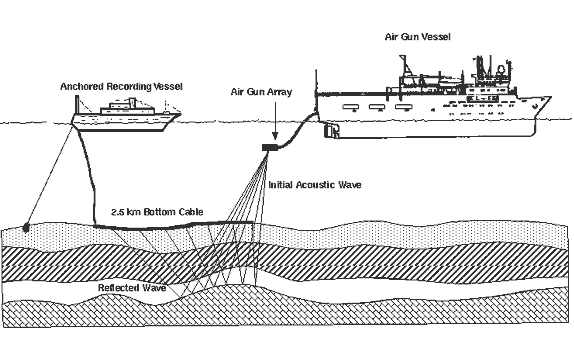
\includegraphics[scale=0.5]{img/Seafloor_Seismic.png}
  \caption{Marine-based Seismic Exploration}
  \label{fig:sea_floor_seismic}
\end{figure}

Geophysics data processing then follows the process of recording the
signals. First of all, multiple steps should be applied to perform the
preprocessing. For example, use the bandpass filter to remove the noise.
And last of all, is the migration step to reconstruct the image of
subsurface.

The detail of how the data are processed is not the topic of this thesis,
so I won't explain it too much. Those who are interested in the subject can
find more information with the help of the search engine. In this thesis, I
only concern about what is relevant with the FPGA implementation of the
computational part, which is explained in next section.

\section{Reverse Time Migration}

In this section, I present a general introduction for Reverse Time
Migration with some seismic terminologies. Revere Time Migration use the
source and recorded signals as input, following a series of computing, then
produce an image of the velocity model, which can maps to the real image of
the interior earth.

You may wonder why the velocity can be mapped to the real constitution of
the interior earth. There are several different objects inside the earth,
such as water, rocks, salt, gas, oil and they are the medium while the wave
propagating through them. The speed of the wave, usually the acoustic wave,
varies from the different medium, for example, the speed of sound is nearly
340 meter per second at temperature 20 degree. If we can generate a model
of the speed inside the earth, we can infer what is inside the earth.

The conventional one-way pre-stack depth migration approach, works well in
the layer medium, shown in Figure (\ref{fig:layer_structure}). If the desired
layer, such as the gas or the oil lies horizontally, it can be easily
discovered with the conventional approach.

\begin{figure}[h]
  \centering
  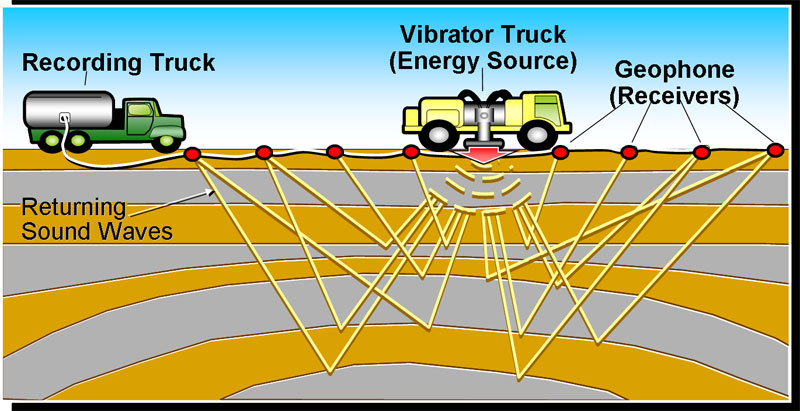
\includegraphics[scale=.45]{img/layer_structure.jpg}
  \caption{Layered structure of the interior earth}
  \label{fig:layer_structure}
\end{figure}

However, not all desired resources are exposed in such a friendly form.
There may be some hill or large rocks beneath the sea, which will obstruct
the desired resource. In addition, some resources will stay in vertical
form or other forms instead of the restrict horizontal form. The
conventional one-way pre-stack depth migration approach could not handle
the previous situation. Thus why Reverse Time Migration emerged.

Reverse Time Migration algorithm is not a new algorithm, instead, it is
first put forward in the 1970s. However, people at that time thinks that it
is impractical or impossible to use such algorithm in practice due to the
tensive  computation requirement. But nowadays, it is impossible to
implement the Reverse Time Migration thanks to the fast developing of
computers.

Instead of just one-way pre-stack depth migration, the Reverse Time
Migration is a two-way pre-stack depth migration, which handles steeply
dipping events, turning waves and multiples. The detail of the algorithm
will be explained in the next section.

Figure (\ref{fig:comparison}) show an introductory example with synthetic
data that illustrates the potential power of the Reverse Time Migration.
There are mainly two part of object in the model, one is water (color from
blue to yellow), the other one is salt (color in red). The figure in the
left is not a real image of the interior earth, but a velocity of that
zone. As the water gets deeper, the speed of the sound becomes faster, so
that is why the color turns from blue to yellow and dark yellow. The salt
is solid object, where the speed of sound is much faster than that in the
water, so the color is in red, a darker color than yellow.

\begin{figure}[h]
  \hfill
  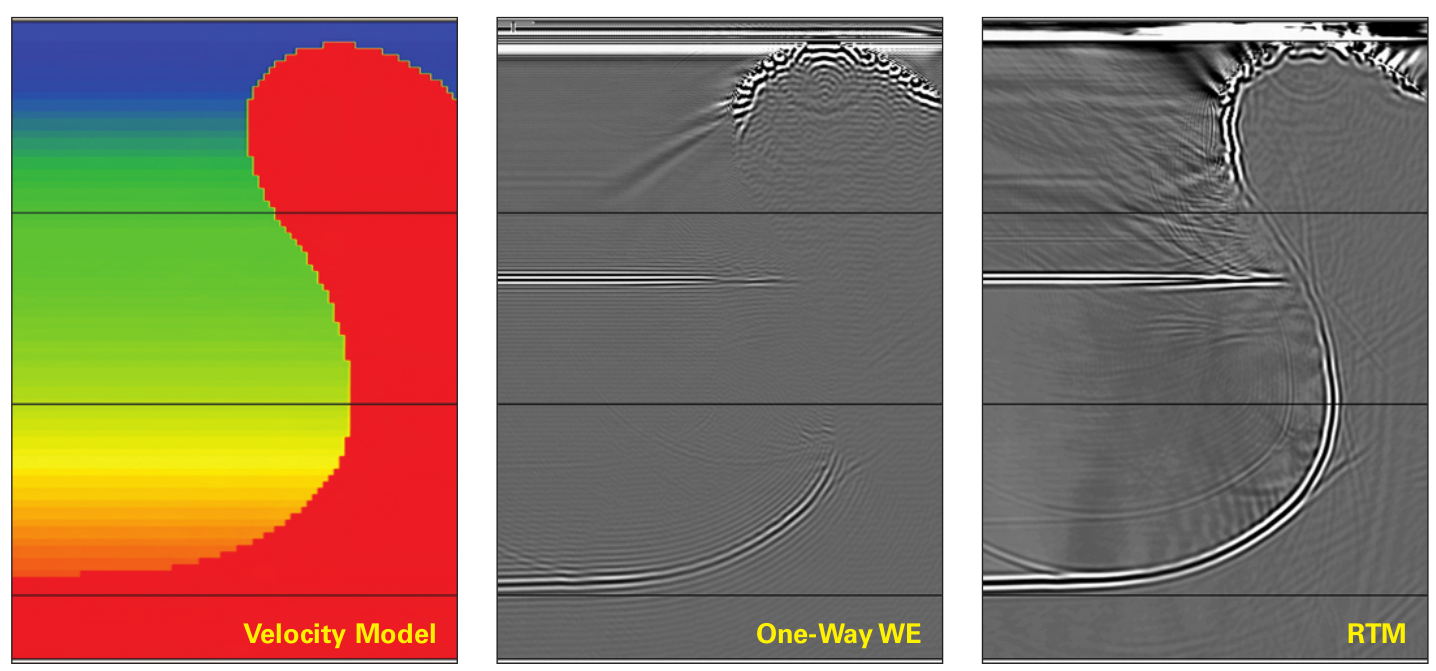
\includegraphics[scale=.25]{img/velocity_model.png}
  \caption{Synthetic comparison of salt flank}
  \label{fig:comparison}
\end{figure}

Concerning about the result, we take a comparison of the middle and right
one in Figure (\ref{fig:comparison}). The middle one is generated using the
one-way wave equation. It is obvious that the salt flank below the overhang
is poorly imaged. On real data, it is difficult to understand the dip and
the structure of sedimentary strata in similar overhang zone. Thus the
potential existence of gas or oil against the salt are impossible to
identify. On the other hand, the last figure, which is produced using the
RTM algorithm, yielding a big improvement. It has a clear profile that is
similar to the original synthetic data.

\section{RTM Algorithm and Analysis}

As it is mentioned in the previous section that the Reverse Time Migration
algorithm can gain a big improvement but it is computationally demanding.
In this section, we have a look at the detail of the algorithm and present
a computation complexity analyze of it.

The main steps of the algorithm is explained as below\cite{rtm}.

\begin{enumerate}
\item the forward extrapolation of a modelled source waved for each shot
  location through a gridded velocity model is performed. And the wave
  field at each time step is saved for later application of the ``imaging
  condition''.
\item the receiver wave field for each shot, which is recorded in the
  field, is backward propagated in time through the same velocity model.
\item at each time step, the corresponding source and receiver wave fields
  are correlated by applying the imaging condition. Thus, the final
  wave field in the source propagating scheme is correlated with the
  initial wave field in the receiver propagation scheme, and so on backward
  through the receiver propagation.
\item the result are summed to form a partial image volume for each shot.
\item the image volumes for consecutive gathers are spatially summed to
  produce the final pre-stack depth image.
\end{enumerate}

So, now you may know why RTM is so computation expensive and has several
decades to be commercially implemented.

\subsection{Mathematical Derivation of RTM}

If we assume that the wave that the wave injects is acoustic wave (sound
wave), then we can use the acoustic wave equation (\ref{eq:acoustic}) as
the first step of the derivation.

\begin{equation}
  \frac{\partial ^2u}{\partial t^2}=c^2 \cdot \left(  \bigtriangledown ^2u \right) +s
  \label{eq:acoustic}
\end{equation}

where \( u = u(x, y, z, t) \) is the pressure field, \(c = c(x, y, z) \) is
the velocity field, \( s = s(x, y, z, t) \) is the source term, and \(
\bigtriangledown ^2 \) is the three dimensional Laplace operator.

The Laplace operator is a second order differential operator in the n-dimensional
Euclidean space, defined as the divergence (\( \bigtriangledown \)) of the gradient
(\( \bigtriangledown f\)). Thus if \( f \) is a twice-differentiable real-valued
function, then the Laplacian of \( f \) is defined by

\[
  \bigtriangleup f = \bigtriangledown ^2 f = \bigtriangledown \cdot
  \bigtriangledown f
\]

Equivalently, the Laplacian of \( f \) is the sum of all the unmixed second
partial derivatives in the Cartesian coordinates:

\[
  \bigtriangleup f = \sum _{i=i} ^n \frac{\partial ^2 f}{\partial x_i ^2}
\]

In particular, if the variable x, y and z denote the three dimensional
Cartesian coordinates, the expansion is:

\begin{equation}
  \bigtriangleup f  = \bigtriangledown ^2 f = \frac{ \partial ^2 f}{\partial x^2} +
                     \frac{ \partial ^2 f}{\partial y^2} +
                     \frac{ \partial ^2 f}{\partial z^2}
  \label{eq:laplacian}
\end{equation}

Thus, replace the Laplacian operator with (\ref{eq:laplacian}), the
equation (\ref{eq:acoustic}) could be derived as:

\begin{equation}
  \frac{\partial ^2u}{\partial t^2}=
  c^2\cdot\left(
  \frac{ \partial ^2 u}{\partial x^2} +
  \frac{ \partial ^2 u}{\partial y^2} +
  \frac{ \partial ^2 u}{\partial z^2}
  \right)
  +s
  \label{eq:acoustic2}
\end{equation}

Equation (\ref{eq:acoustic2}) can be further factored as:
\begin{equation}
  \frac{u_{t+1} - 2u_{t} + u_{t-1}}{dt^2}=
  c^2\left(
  \frac{ \partial ^2 u}{\partial x^2} +
  \frac{ \partial ^2 u}{\partial y^2} +
  \frac{ \partial ^2 u}{\partial z^2}
   \right)
  +s
  \label{eq:acoustic3}
\end{equation}

Then we introduce a method called \emph{stencil}, which is a geometric
arrangement of a nodal group that relate to the point of interest by using
a numerical approximation routine in mathematics, especially the areas of
numerical analysis concentrating on the numerical solution of partial
differential equations. The derivation of stencil from the second order
partial difference is in appendix. Now, equation (\ref{eq:acoustic3}) could
be written as:

\begin{equation}
  \frac{u_{t+1} - 2u_{t} + u_{t-1}}{dt^2}=
  c^2 \cdot\left( \frac{1}{dh^2} \cdot stencil\left( p_t \right) \right)
     +s
  \label{eq:acoustic4}
\end{equation}

where \( dh \) is the distance between the two neighbours of the stencil
operation. For a specific point x, the stencil result of that point in 6th
order is:

\begin{equation}
  \begin{split}
    {f(x)}'' =
    & w_{-3}f\left( x - 3 \Delta x \right) +
      w_{-2}f\left( x - 2 \Delta x \right) +
      w_{-1}f\left( x - \Delta x   \right) + \\
    & w_{0}f\left( x \right) + \\
    & w_{1}f\left( x + \Delta x \right) +
      w_{2}f\left( x + 2 \Delta x \right) +
      w_{3}f\left( x + 3 \Delta x \right)
  \end{split}
\end{equation}

where \( \Delta x \) has the same meaning with \( dh \) in equation
\ref{eq:acoustic4}. To give a better vision, Figure
\ref{fig:6th_order_stencil_1d} give a outline of one dimensional stencil.

\begin{figure}[h]
  \centering
  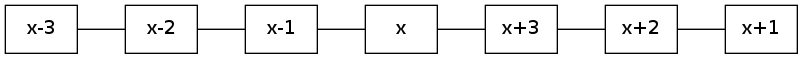
\includegraphics[scale=0.4]{img/6th_order_stencil.png}
  \caption{6th order one dimensional stencil}
  \label{fig:6th_order_stencil_1d}
\end{figure}

Figure (\ref{fig:6th_order_stencil_1d}) give us a array like presentation of
1D stencil, and the result at element i is:

\[
  y\left[ i \right] = c_3  x\left[ i-3 \right] +
                      c_2  x\left[ i-2 \right] +
                      c_1  x\left[ i-1 \right] +
                      c_0  x\left[ i \right] +
                      c_1  x\left[ i+1 \right] +
                      c_2  x\left[ i+2 \right] +
                      c_3  x\left[ i+3 \right];
\]

where \( c_0 \) to \( c_3 \) are dedicated coefficients based on the
different order of the stencil.

In the previous acoustic equation, the stencil is a 6th order 3D stencil,
which is denoted by x, y and z axis. Thus, given a point (x, y, z), there
are 18 (3 x 6) points around and the center point, 19 points altogether,
will be used to perform the calculation. Figure
(\ref{fig:6th_order_stencil_3d}) gives a sketch of such stencil.

\begin{figure}[h]
  \centering
  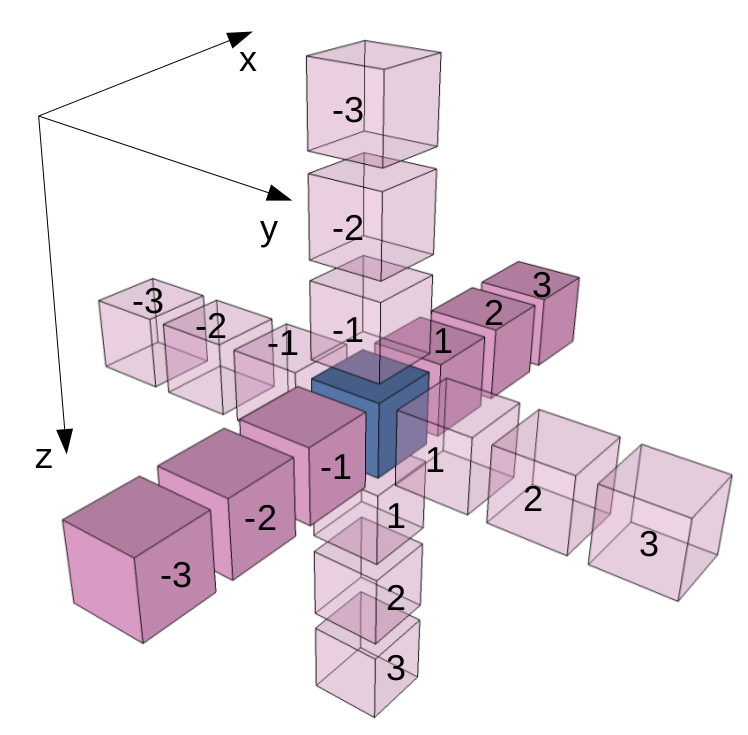
\includegraphics[scale=0.4]{img/stencil_6_3d.png}
  \caption{6th order 3 dimensional stencil}
  \label{fig:6th_order_stencil_3d}
\end{figure}

The calculation of the stencil in Figure (\ref{fig:6th_order_stencil_3d})
is sum of the x, y and z axis. We can draw a formula to denote it.

\begin{equation}
  g(x,y,z) = \sum _{i=-3} ^{+3} w_i  f(i,y,z) +
             \sum _{j=-3} ^{+3} w_j  f(x,j,z) +
             \sum _{k=-3} ^{+3} w_k  f(x,y,k) -
             2f(x,y,z)
 \label{eq:stencil_3d}
\end{equation}

Changing the equation (\ref{eq:stencil_3d}) to the programming psudo-code
is very convenient for programming to code. Listing (\ref{lst:stencil_code_1element})
shows the desired psudo-code.

\begin{figure}
\centering
\lstinputlisting[
  caption={Pseudo code of calculating one element using stencil method},
  label={lst:stencil_code_1element}
  ]
  {code/stencil_1elem.c}
\end{figure}

Listing (\ref{lst:stencil_code_1element}) only works for 1 element in the
array. In practice and in the previous equation (\ref{eq:acoustic}), all
the elements in the three dimension volume should be calculated one by one
except for the boundaries. Thus the complexity of calculating the stencil
in a volume is \BigO{n^3}

Each step of the iteration, what we desire is to calculate the the wave
field of time \( t + 1 \), moving the item \( t \) and \(t-1\) to the right
side of the assignment operator of equation \(\ref{eq:acoustic4}\), we get
the equation (\ref{eq:acoustic5}).

\begin{equation}
  u_{t+1} =
  2u_{t} - u_{t-1} +  dt^2 \left( c^2\cdot\left( \frac{1}{dh^2} \cdot stencil\left( p_t \right) \right)
 +s_t\right)
  \label{eq:acoustic5}
\end{equation}

Now, it is easy to write the pseudo code of coressponding to the equaltion
(\ref{eq:acoustic5}). Storing the wave field in a 4 dimensional array,
including t, x, y, and z dimension. s is also a one dimensional array
storing the the source signal. The psedo code is shown in Listing
(\ref{lst:acoustic}) in page \pageref{lst:acoustic}.

\begin{figure}
  \centering
  \lstinputlisting[
    caption={Pseudo code of calculating forward acoustic wave equation},
    label={lst:acoustic}
  ]
  {code/acoustic.c}
\end{figure}

As you can see, the array u is a four dimensional array. If the nz = ny =
nx = 512, and nt = 500, the size of the array is \( 512^3 * 500 * 4 =
268435456000 \) bytes, that is 250G, which is impossible to store in the
memory. However, the size of the array is much smaller than that in the
reality, because assuming that dt = 0.002, nt = 500, dh = 20, it is recorded for
only 1 second of sound for the cude of 10240m * 10240m * 10240m, nearly a
cube of 10km for a single shot.

What's worse, the algorithm listed in Listing (\ref{lst:acoustic}) is only
part of the RTM algorithm. The Reverse Time Migration algorithm is a
two-way pre-stack depth migration, which is explained in the previous
section, the wave propagation of the source and receiver should be
correlated, to gain the resulting image. The pseudo code\cite{fu11} is shown in
Listing (\ref{lst:rtm}) in page \pageref{lst:rtm}.

\begin{figure}[h]
  \centering
  \lstinputlisting[
    caption={Pseudo code of the RTM algorithm},
    label={lst:rtm}
  ]{code/rtm.c}
\end{figure}

\subsection{Complexity analyze}

Dablain (1986) effectively applies explicit high-order finite
difference spatial derivatives to the acoustic wave equation.
We also apply high-order spatial derivatives to the acoustic
wave equation. Using the \( 2^{nd} \) in space finite differences, the
forward and backward wave field propagations can be calculated as
\cite{rtm_psdm}:

\begin{equation}
  u ^{l(+/-)1} _{i,j,k} = 2u^l _{i,j,k} - u^{l(+/-)1} _{i,j,k} + \Delta t^2
  c^2 _{i,j,k} (\left( \bigtriangledown ^2 u ^l _{i,j,k}  \right) ^ n_0 +
  s ^l _{i,j,k})
\end{equation}

where

\[u^l _{i,j,k} = u(i\Delta x, j \Delta y, k \Delta z, l \Delta t),\]
\[ s^l _{i,j,k} = s(i\Delta x, j \Delta y, k \Delta z, l \Delta t),\]
\[ c_{i,j,k} = u(i\Delta x, j \Delta y, k \Delta z), \]

and \( \Delta t \) =  the temporal step size for finite differencing, \(
\Delta x \), \( \Delta y \), and \( \Delta z \) are the spatial sampling
intervals, and \( \bigtriangledown ^2 u^t _{x, y, z} \) the Laplacian
calculated with \( n^{th} \) order of accuracy at each time step t,
centered at an x-, y-, and z- location. During the backward extrapolation
the source
term is replaced by the recorded input data. The Laplacian with
\( n^{th} _0 \) order accuracy can be given by ().

\begin{equation}
  (\bigtriangledown ^2 u ^l _{i,j,k})^n_0 = w_0(\frac{1}{\Delta x^2} +
  \frac{1}{\Delta y^2} + \frac{1}{\Delta z^2})u^l _{i, j, k} + \Phi
\end{equation}

where

\begin{equation}
  \begin{split}
    \frac{\Phi}{\sum_{m=1} ^{n_0 / 2}w_m} =
      &\frac{1}{\Delta x^2}\left(u^l _{i-m, j, k}+ u ^l _{i+m, j, k}
      \right) + \\
      &\frac{1}{\Delta y^2}\left(u^l _{i, j-m, k}+ u ^l _{i, j+m, k}
      \right) + \\
      &\frac{1}{\Delta x^2}\left(u^l _{i, j, k-m}+ u ^l _{i, j, k+m} \right)
  \end{split}
\end{equation}

where w are finite differencing coefficients of the desire
accuracy. Coefficients are calculated via a series expansion
method. For example, if a second derivative of a function
\( f(x) \) is required to be approximated with \( 6^{th} \) order accuracy
on a uniform grid, the approximation can be written as:

\begin{equation}
  \begin{split}
    {f(x)}'' =
    & w_{-3}f\left( x - 3 \Delta x \right) +
      w_{-2}f\left( x - 2 \Delta x \right) +
      w_{-1}f\left( x - \Delta x   \right) + \\
    & w_{0}f\left( x \right) + \\
    & w_{1}f\left( x + \Delta x \right) +
      w_{2}f\left( x + 2 \Delta x \right) +
      w_{3}f\left( x + 3 \Delta x \right)
  \end{split}
  \label{eq:finite}
\end{equation}

Finite difference weights in (\ref{eq:finite}) can be calcuated using a
series expansion method. The coefficients are symmetrical around \( w_0 \)
for a uniform grid.

The cost of the method is approximately given by the following equation:

\begin{equation}
  C_e \approx 2n_t n_x n_y n_z \left( 3n_0 + 19 \right)
  \label{eq:complexity}
\end{equation}

Where \( C_e \) is the number of floating point operations; \( n_t \) is
the number of time steps; \( n_x , n_y , n_z \) are the number of samples
in the x, y and z directions.

So equation (\ref{eq:complexity}) is similar for the algorithm in Listing
(\ref{lst:rtm}) in page \pageref{lst:rtm} for only a single shot. Adding
the number of shots to the complexity, equation (\ref{eq:complexity})
become (\ref{eq:complexity2}).

\begin{equation}
  C_e \approx 2n_s n_t n_x n_y n_z \left( 3n_0 + 19 \right)
  \label{eq:complexity2}
\end{equation}

It is almost unable to calculate such a algorithm in general purpose 
computer in a short time. What's more, the memory can not satisfy the 
requirement. The size of cache in the general purpose computer or some advanced 
server is usually several mega bytes. It is rather small compared with the 
size of the wave field array. The use of cache doesn't gain much in this 
application.

\section{Implementation of RTM} % (fold)

\label{sec:Implementation of FPGA}

The paradigm of coding in FPGA is different from that in general purpose
coding, such as C/C++. To be more precise, it is called describing rather
than coding. Imaging the data flowing through the chip, and you are
designing a filter in the chip that can make some operation on the data.

When you are designing the kernel with Java, the code that you write
doesn't have a directly impact to the configuration of FPGA. Instead, the
Maxcompiler will endeavor to figure out the meaning of the code, or the
logic of the code, and the compiler will then generate the hardware
description language for the chip. So, you can also be convinced that you
are communicating with the compiler, rather than the chip directly.

\subsection{Streaming in FPGA} % (fold)
\label{sub:Streaming in FPGA}

To have the whole array processed, the host program (c/c+) usually use the
for loop to iterate through each element: make action to the element, and
then iterate next one. Such a loop is replaced by the streaming concept of
FPGA. So you don't need to write loop in the FPGA kernel design. You only
need to design the filter filtering each element.

Here I present a basic example of kernel designing to illustrate the
concept of FPGA designing, or paradigm. If we want to make a linear
transformation (equation (\ref{eq:fx})
to a vector, that is, to each element to the vector, a single for loop will
intuitive come to our mind.

\begin{equation}
  f(x) = 2x + 3
  \label{eq:fx}
\end{equation}

The pseudo code is shown in Listing (\ref{lst:fx}), which is unnecessary to
to explain. In this example, each element is applied to the function
(\ref{eq:fx}). The first element is processed first, then the second one,
and next and next. It is controlled with the help of the \emph{for} loop.
In FPGA kernel designing, data are streamed to the kernel, one by one. So
we don't have to write the for loop explicitly, instead, we are only
concentrate on the filter (in this example, the transformation).

\begin{figure}
  \centering
  \lstinputlisting[
    caption={Pseudo code of the transformation \( f(x) = 2x + 3 \) to a
    vector},
    label={lst:fx}
  ]{code/fx.c}
\end{figure}

Thus the first thing to do while designing the FPGA kernel is to specify
the input stream where the data from one by one and output stream where the
data goes one by one. We can achieve it using the given API. The core of
the kernel is designing how each data should processed, in this example,
that is the simple transformation. The code snippet is shown in listing
(\ref{lst:fx_kernel}).

\begin{figure}
  \centering
  \lstinputlisting[
    caption={Code snippet of the FPGA kernel of transformation to a
    vector},
    label={lst:fx_kernel},
    language={java}
  ]{code/fx_kernel.java}
\end{figure}

As you can see from the code snippet of the kernel, which is written in
Java, that there is no loop through out the kernel. The only one controlled
instruction is the transformation listed in line 9. The concept
\emph{streaming} is really import in FPGA designing because we are
designing a circuit, in particular, we are connecting the wires of the
circuit. In this example, we need an electrical element to perform the
multiplication and an element to perform the addition. These requirement
are issued by only one line of code (line 9). Then the Maxcompiler will
generate the target code, the hardware description code. So, in my
opinion, we are talking to the Maxcompiler and the Maxcompiler will make
a translation for us. Figure (\ref{fig:fx}) shows a graphical representation
of this kernel.

\begin{figure}
  \centering
  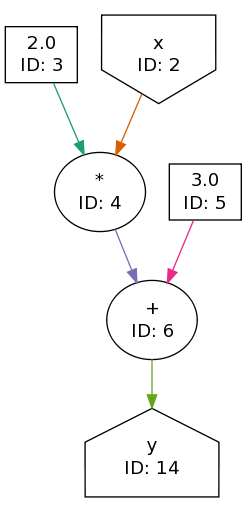
\includegraphics[scale=0.5]{img/SimpleKernel_original.png}
  \caption{Graph for a simple kernel}
  \label{fig:fx}
\end{figure}

In most cases, designing a kernel is not as simple as the previous example,
especially when the data to the stream is not independent. Most of time,
the FPGA designer are analyzing the algorithm and trying to cut the
relationship between the data. The more independent of the data, the easier
to design the kernel.

% subsection Streaming in FPGA (end)

\subsection{1D stencil design in FPGA} % (fold)
\label{sub:1D stencil design in FPGA}



The performance of the stencil operation is the key to the performance to
the whole application, as the RTM algorithm keeps calculating the stencil
operation. To have a better understanding of FPGA designing, we consider
the 1D-stencil design in FPGA rather diving into the 3D-stencil.

Apart from the previous example, which is only a simple transformation to
one element of the vector, where each element is independent, the neighbors
of the element is required to perform the stencil action. However, the
element is streamed to the kernel for each cycle. So, the point is, how to
attract the data that is in the future or in the past.

Stream offsetting allows us to access data elements within a stream
relative to the current location\cite{maxcompiler_tutorial}. The distance
from the largest to the smallest offset forms the window of data that must
be held on the FPGA on-chip memory. What's more, the core concept of stream
computing is operating on windows into data streams. Not only does the data
window is held in on-chip memory on the FPGA, and the data items are held
on-chip for exactly the amount of time required. This means good use of
on-chip memory use, since data is held for only so long as it is needed
rather than reload. And it also means good use of on-chip memory capacity,
since the data is held for only so long as it is needed.

\begin{figure}
  \centering
  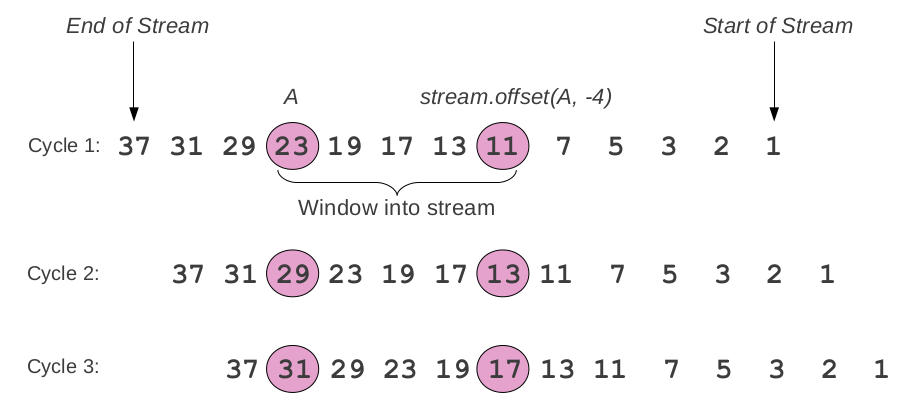
\includegraphics[scale=0.4]{img/window.png}
  \caption{Stream offsets from a window into a data stream}
  \label{fig:stream_window}
\end{figure}

Figure (\ref{fig:stream_window}) show a data stream A over three cycles.
The first element of the stream is 1, and the last element of the stream is
37. The current location will move from one location to next of each cycle.
Now, the current location (head of the stream) is A, which has the value
23. A kernel program accessing the head of the stream and also a data item
four elements into the past (with a value of 11 in cycle 1) create a window
of size five into stream A. Each cycle, the data in the stream moves
through the window.

\begin{figure}
  \centering
  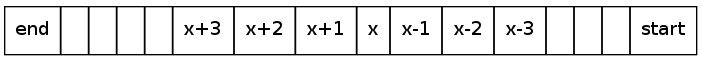
\includegraphics[scale=0.5]{img/array.png}
  \caption{Points for 1D array for stencil operation}
  \label{fig:array}
\end{figure}

\begin{figure}
  \lstinputlisting[
    caption={Code snippet for 1D stencil using stream offset technique},
    label  ={lst:1d_stencil}
  ]{code/stencil1d.java}
\end{figure}

Any conventional array operation can be expressed in terms of stream
offsets. In this subsection, we consider the 1D convolution. Figure
(\ref{fig:array}) shows one way in which the collection of points for
stencil operator can be expressed in terms of offsets. The current position
(head of the stream) is A, the other points (three from the future and
three from the past) are needed to the stencil operator. Each element
including those from the future and the past are accessed using the stream
offset technique. Listing (\ref{lst:1d_stencil}) gives a code snippet of 1D
stencil kernel designing.


% subsection 1D stencil design in FPGA (end)

\subsection{Forward Migration } % (fold)
\label{sub:Forward Migration }

There are two parts of Reverse Time Migration, the first part is
\emph{forward migration} and the second part is \emph{reverse migration}.
The calculation logic is nearly the same except that the forward migration
mimic the wave field propagation from time \( t=t_0 \) to \( t=t_n \) while
the reverse migration mimic the wave field propagation from the reverse,
that is, from time \( t = t_n \) to \( t = t_0 \). They cannot be
implemented in a single loop because in the reverse migration, we need to
calculate the product of wave field at time t, which is shown at line 40 in
Listing (\ref{lst:rtm}) in page \pageref{lst:rtm}. Reviewing Listing
(\ref{lst:rtm}) in page \pageref{lst:rtm} again reveals that the core
implementation of the first outer loop and the second outer is similar. So,
only one design of the kernel is enough for calculating both forward
migration and reverse migration.

\begin{figure}
  \centering
  \lstinputlisting[
    caption={Pseudo code in FPGA implementation},
    label={lst:part_of_forward_modeling}
  ]{code/part_of_forward_modeling.c}
\end{figure}

The timestamps control is handed to the host code while passing the
remaining forward modeling (stencil operation plus some additional
calculation) to the FPGA kernel. The kernel need to implement the pseudo
code in Listing (\ref{lst:part_of_forward_modeling}).


\subsubsection{Transform The Loops} % (fold)
\label{ssub:Transform the lo}
It is a very simple control statement in the host code, but it is not in
the FPGA implementation. As you are designing the logic of FPGA, connecting
the wires in the configurable logic unit, and the data streams to the FPGA,
there is no \emph{for} loops and no \emph{if} branches. We need to find
some alternatives to implement the same function.

As for the loops, the stream offset can be used to access the elements
in the past or at the future, which is explained in  the previous
subsection. However, in this part, we need to mimic the nest loop
controlling but what we explained is the single loop rather than the
nest loops. Is there any ways to mimic the nest loop in the FPGA kernel?

The nest loop is used to access the elements in the cube, a 3D array. If we
stretch the 3D array to a 1D array, which is similar to treat the 2D array
as a 1D array, accessing the elements through manually calculated index
rather than the array indexes, we can mimic that nest loops with simple
stream offset in FPGA kernel. However, there are more than one operation
rather than only the accessing operation. We still need to test if the
current element is at the boundary, which is nearly impossible to mimic the
branch conditional test with 1D array. For example, if the boundary is
inner three layers and outer three layers, how could you calculate the
index in a 1D array?

There is another technique called counter, which can be used to mimic the
nested for loop. We can control the behaviors of the counter such as the
increment value, the start value, the wrap value and the wrap mode. In this
specific question, we use three counter to mimic the nested loop. The
detail is explained.

\begin{enumerate}
  \item we use the first counter, named \emph{counterX} to mimic the
    behaviors of \emph{ix}, the start value of the counter is 0, and the
    counter increase by 1 at each cycle until it reach the value \emph{nx -
    1}, then it wrap to 0 again and continuing the counting. So the counter
    will keep counting from 0 to nx - 1, and back to 0 to nx-1.

  \item the second counter, named \emph{counterY}, is used to mimic the
    behavior of \emph{iy}. Of course the counter cannot keep increasing
    at every cycle, instead, it only increase 1 when the \emph{counterX}
    wrap. \footnote{wrap means that the counter reach the max value and
      count back from the start value. In this case, it refers that the
    counterX reach nx - 1 and count back to 0}. Identifying the behavior
    of the counter, we can determine when to enable the \emph{counterY}
    and when to disable it. It is only enable when \emph{counterX}
    wraps. The remaining behaviors is similar to the \emph{counterX},
    start counting from 0 to ny - 1 and wrap to 0.

  \item the third counter, named \emph{counterZ}, which mimic the behavior
    of \emph{iz}. The counter is similar to \emph{counterY}. It is enabled
    when \emph{counterY} wraps.

    \item at every cycle, we can get the value of the counters, which is the
      same as ix, iy and iz, to perform the calculation and branch testing.

\end{enumerate}

% subsubsection Transform the lo (end)

\subsubsection{Transform The Branches} % (fold)
\label{ssub:Transform The Br}
Another question is how to mimic the logical \emph{if/else} branch in the
kernel. The \emph{if/else} statement is part of the high level language,
such as C/C++. But What's the underlining implementation of them? In the
hardware design, a multiplexer is used to select one of the two input in
terms of the controlling signal, the predicate. When  the predication
is compound predication, where is controlled by the logical AND (\&\&) or
logical OR, (||) operator, we have to use alternatives to replace them,
because in the hardware designing, there is no logical AND (\&\&) and
logical OR (||)
operators, because it is impossible to replicate th conditional evaluation
(or ``short-circuiting'') semantics in a data flow kernel. We can use the
bit-wise OR (|) and bit-wise AND (\&) to replace them.
% subsubsection Transform The Br (end)

\subsubsection{Additional Improvement} % (fold)
The main part of design is described in the previous subsection, it is not
feasible enough however, because most of the dimension, or the coefficients
are hard coded in the kernel. Building the kernel in the FPGA hardware
takes lots of time, from hours to weeks, so it is important to build a
kernel that is flexible enough. The users can provide the parameters
through the host code for each run, thus the users can run FPGA kernel
multiple time with different parameter with only one hardware build. Those
technique includes \emph{scalar input}, \emph{variable stream offsets},
\emph{dynamic stream offsets} and \emph{controlled input/output}. The usage
is not discussed in this article. Those who are interested in can refer to
Dataflow Programming with MaxCompiler\cite{maxcompiler_tutorial}.

\label{ssub:Additional improvement}

% subsubsection Additional improvement (end)

% subsection Forward modeling implement (end)

\subsection{Reverse Migration} % (fold)

Reverse Migration is the second part of Reverse Time Migration. We adjust
the input of the kernel and control the timestamps. In this part, we can
use the same kernel as that is used in the forward migration. It is the 
most important part of the algorithm because it is responsible for 
generating the image of the subsurface. 

The computation complexity is the same as the forward migration, but the 
data varies. The result wave fields of the forward migration should be 
kept, because they are needed in this step. The most 
computationally-demanding part has handed over to the FPGA kernel, which is 
the same as the previous one. The host code set the different the input 
streams and coefficients for both forward migration and reverse migration. 
So, more work is controlled by the host code.

\label{sub:Reverse Mi}

% subsection Reverse Mi (end)
% section Implementation of FPGA (end)

\section{Results And Comparison} % (fold)

Given there there is an version of Reverse Time Migration algorithm
that is implemented on CPU as the benchmark, the comparison is the
running performance (time) between on CPU and FPGA. Of course, the
most essential and important thing is to ensure the correctness of
the implementation of FPGA, which is done by compare the output image
(cube) of CPU and FPGA cell by cell when they accept the same input
data.

In my implementation, the single precision floating point\footnote{32
bit, 8 bit for exponent and 23 bit for mantissa} is used, so the difference
of the two cell is \( \epsilon=10^{-23} \)
. If the difference of the cells on CPU and FPGA in the same location
within the \( \epsilon \)
, we treat the two floating point values identical. If each cell in
CPU and GPU is identical, the whole image are the same. Thus proving
the correctness of FPGA implementation.

Given that the implementation of RTM algorithm is correct, I endeavor
to compare the performance between the two implementation. There are
several parameters impacting the required running time, including
the number of shots, the number of time steps and the size of the
cube. In this section, I compare the performance within one shot,
because the running time is linear to the number of shots. I compares
the running time when the size of cube varies first, and then compare
the consuming running when the number of time steps varies.

\subsection{Platform Information} % (fold)

In this subsection, the platform for both the CPU and FPGA is introduced.
The comparison in the rest of this section is operated on i7 CPU,
which includes 8 cores, with the frequency of each core 2.93GHz. The
FPGA used in this implementation is a \emph{Xilinx V6-SXT475} whose
frequency is about 100MHz. Figure (\ref{fig:Platform-information-of})
shows the detail information of the host (CPU) and device (FPGA).

\begin{figure}
\begin{centering}
\begin{tabular}{|c|c|c|}
\hline
 & Host (CPU) & Device (FPGA)\tabularnewline
\hline
\hline
OS & Linux 2.6.18 & Maxeler OS 2011.3.1\tabularnewline
\hline
Compiler & GCC & MaxCompiler\tabularnewline
\hline
Processor & Intel(R) Core(TM) i7 & Xilinx V6-SXT475\tabularnewline
\hline
Freq & 2.93GHz & 100MHz\tabularnewline
\hline
RAM & DDR3 16G & DDR3 24G\tabularnewline
\hline
\end{tabular}
\par\end{centering}

\caption{\label{fig:Platform-information-of}Platform information of host and
device}


\end{figure}

To record the running time, the Unix API \emph{gettimeofdate()} is preferred
to the \emph{clock()} function in C library because the
\emph{clock()} function may make some mistake while the code is running on
the device. The time that is recorded by \emph{gettimeofdate()} is similar
to the wall clock.

\label{ssub:Platform information}


\subsection{Running Time vs. Cube Size}
\label{sub:Running Time vs. Cube Si}

% (fold)

\begin{figure}
  \centering
  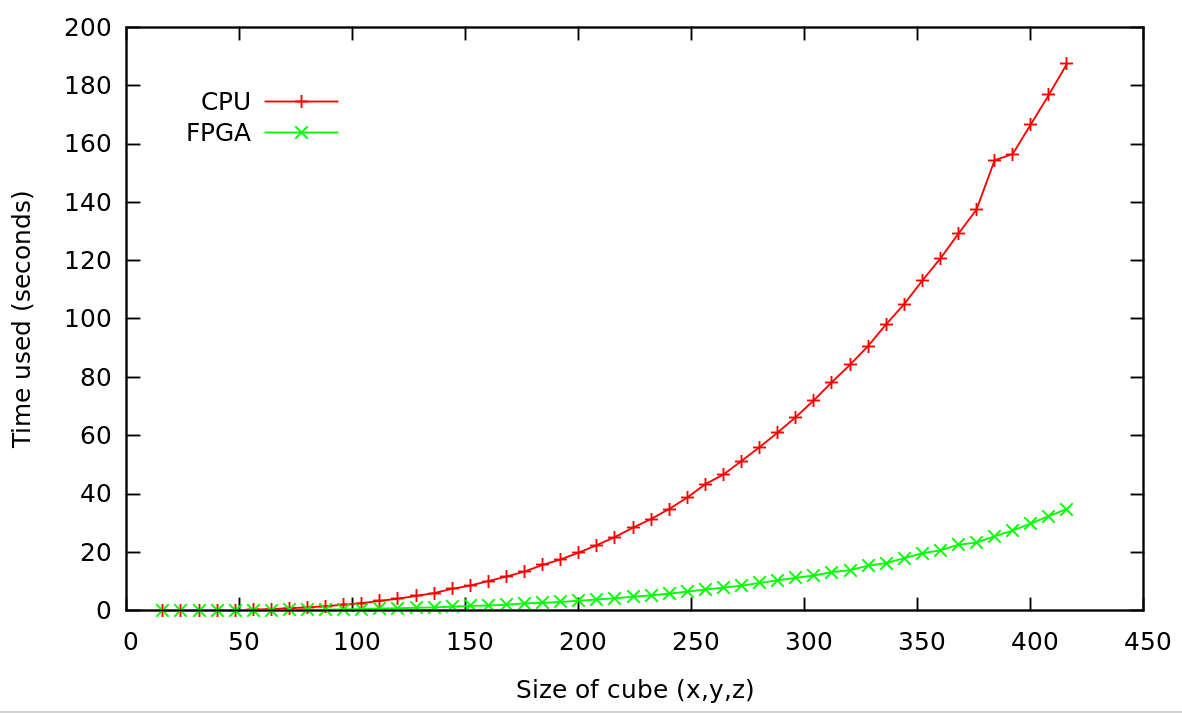
\includegraphics[scale=0.3]{img/t10size16to256.png}
  \caption{Comparison of time used between CPU and FPGA when size varies}
  \label{fig:comparison_1}
\end{figure}

The cube size, the array that used for iterating, represents the size
of the seismic exploration. Given \ensuremath{dx=20m}
 and the cube is a \ensuremath{32\times32\times32}
 array, the practical size in reality is a cube whose edge is 640m
long, which is fairly small. The smaller value of dx is, the higher
the resolution is. However, we need to change expand the size of the
array to gain the same practical size if we decrease the value of
dx.

Given that the number of time steps is 10, which is a fairly small number
purely used for simulation, but in reality, its range is between thousands
to hundred of thousands, while the size of the cube varies, from 32 to 416.
Figure (\ref{fig:comparison_1}) depicts the running time used by them.

It shows that when the cube is
small, calculation in FPGA may take larger amount of time than that in CPU
because data in the host memory need to be transferred to the device, and
the transfer the data back to the host when the core calculation is done.
However, as the size of the cube increase, the host needs more and more
time than the device. In typical, the calculation time needed by the CPU is
conform to function \( f(x) = ax^3 \) because complexity of the algorithm
in the inner stencil operation is \(O(n^3)\) while it is not in FPGA.

Another point that affects the running time of the host code is the cache.
When the size is small, part of the data can be stored on the cache of the
CPU, resulting fast speed in the host code. However, when the size of the
cube increase, the cache cannot hold the whole array, even only part of the
array, thus increasing the miss rate for the cache indexing.

The bandwidth of PCI express and the frequency of FPGA affect the
calculation speed of FPGA. In the current implementation, no optimization
is applied to the FPGA kernel design. So the resource usage is quite low,
neary 6.89\% of Look Up Table (LUT), 3.89\% of Flip Flops (FF) and 1.59\%
of Digital Signal Processor (DSP). Lots of work can be done in the
optimization of the kernel, but it is not discuss in this thesis.

\begin{figure}
  \centering
  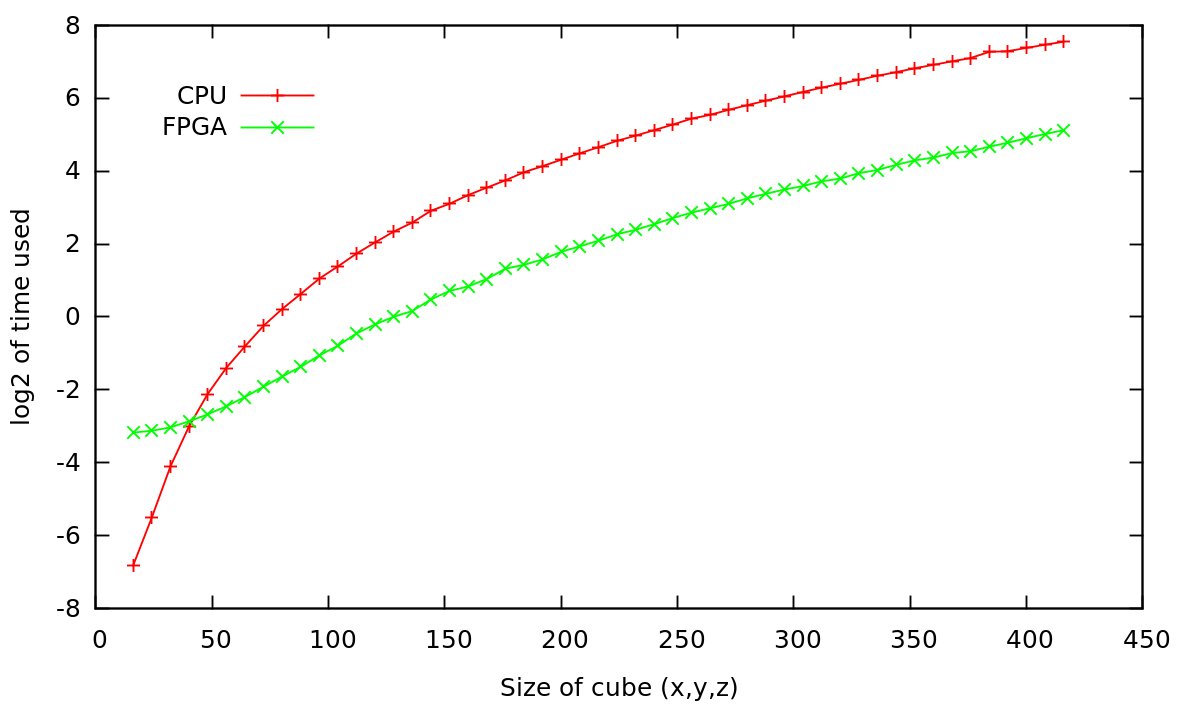
\includegraphics[scale=0.3]{img/t10size16to256_log.png}
  \caption{Transform time t to log(t), then compare them}
  \label{fig:comparison_2}
\end{figure}

To have a deeper understanding to the time used in both CPU and FPGA,
Figure (\ref{fig:comparison_2}) transform the time used \( t \) in each
point to \(\log_2\left( t \right) \). So it is easy to identify the details
when the size of the cube is small. Figure (\ref{fig:comparison_2}) shows
that time consumed by CPU is less than that by FPGA when the size is less
than 50. That is because the data should be transferred to FPGA through PCI
Express and be transferred back from the device after the calculation.
On the other hand, the CPU can make full use of cache when the size of the
array is small, resulting in relative high cache hit rate.

% subsection Running Time vs. Cube Si (end)

\subsection{Running Time vs.  Time Steps} % (fold)

\begin{figure}[h]
  \centering
  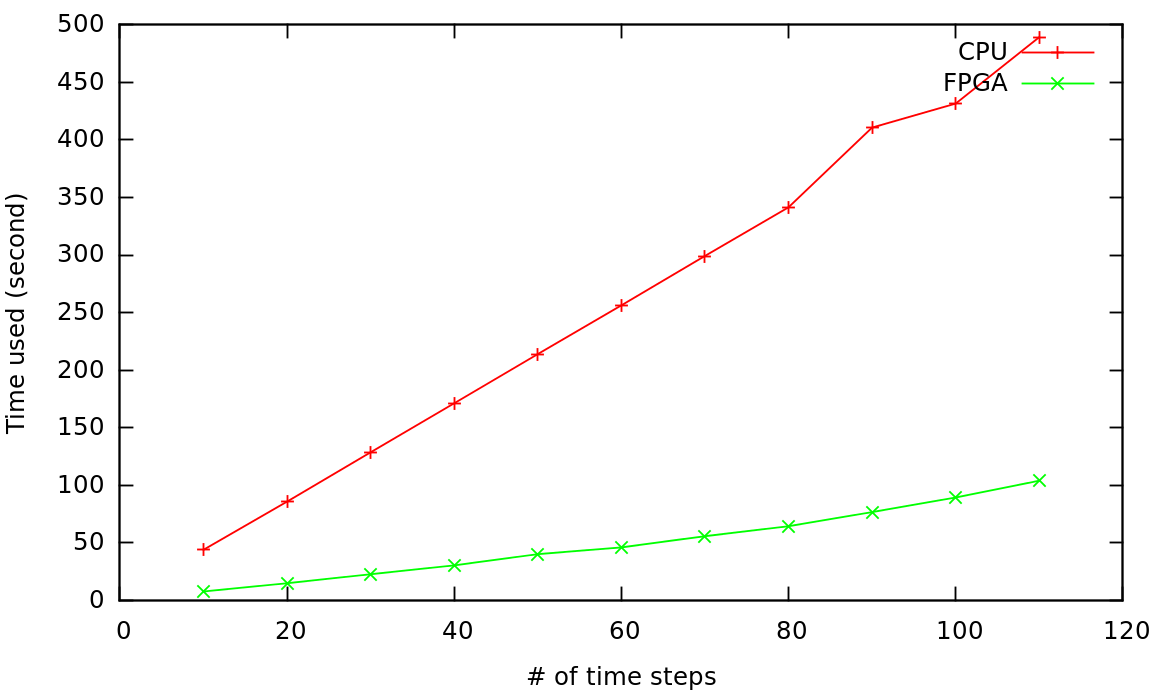
\includegraphics[scale=0.32]{img/size256t10to110.png}
  \caption{Comparison of time when time steps varies}
  \label{fig:comparison_3}
\end{figure}

It is a good idea to let only one parameter varies while keeping others
still. So this time, we keep the size of the cube as \( 256 \times 256
\times 256 \) and let the number of time steps varies. Figure
(\ref{fig:comparison_3}) depicts the relation between the running time and
the number of steps of both CPU and FPGA. The shape of the CPU line is 
pseudo-linear, because as the number of time steps increase, the cache hit 
rate will decrease and miss rate will increase, resulting in high memory 
accessing latency, which will decrease the total computational time 
dramatically. The running time of FPGA is relatively stable than that of 
CPU, and its slope is much gentle than that of CPU's. The FPGA takes about 
100 second to make the wave field propagate for 110 steps while the CPU 
needs about 500 seconds to do the same task. 

The number of time steps 
varies from thousands to tens of thousands in practical, and the size of 
the cube is about hundreds of GB or TBs, which is nearly impossible to 
store them in local memory. But it is feasible to implement it on FPGA 
because once the kernel is designed, the data will flow to the kernel 
element by element like streams. Part of the data can flow to the kernel 
first, and then follows another part of the data.

% section Performance comparison (end)

\section{Conclusion} % (fold)
\label{sec:Conclusion}

This thesis presents Field Programmable Gate Array (FPGA) designing with 
the help of Maxeler OS and Reverse Time Migration (RTM) algorithm, which is 
the most computationally demanding algorithm in oil and gas exploration 
operations. In addition, the thesis presents FPGA-based solution for the 
RTM algorithm.

By utilizing the reconfigurability of the FPGA device, my RTM design 
manages to speed up the calculation in term of the hardware calculation 
instead of software calculation. When comparing to Intel(R) Core(TM) i7 
CPU, the naive implementation of FPGA achieves 6X speed up without any 
optimization. 

I think FPGA is becoming efficient High Performance Computing solution, 
which is an alternative to conventional CPU and GPU, because it has 
abundant computation and storage resources on the board. What more, 
paralleling the FPGA kernel by utilizing more FPGA resource is a good way to 
optimize the FPGA kernel, which will result in better performance. 
Meanwhile, users can provide other boost to the performance as they can 
perform customization on various aspect of the design. These unique 
properties makes FPGAs a preferable choice for many 
computationally-intensive application.

% section Conclusion (end)

\begin{thebibliography}{9}
  \bibitem{fu11} H. Fu and R. G. Clapp, \emph{Eliminating the memory
    bottleneck: an FPGA-based solution for 3d reverse time migration,}
    in Proceedings of the 19th ACM/SIGDA international symposium on Field
    programmable gate arrays, 2011, pp. 65-74.

  \bibitem{herb11} Herb Sutter, \emph{The Free Lunch Is Over: A Fundamental
    Turn Toward Concurrency in Software,} Dr. Dobb's Journal, 30(3), March
    2005. Retrieved 21 November 2011.

  \bibitem{yoon03} K. Yoon, C.Chin, S. Suh, L. Lines, and S. Hong.
    \emph{3D Reverse-time Migration Using the Acoustic Wave Equation:
    An Experience with the SEG/EAGE Data Set.} The Leading Edge, 22(1):38-41,
    2003.

  \bibitem{moore}
    \emph{Moores law, Wikipedia, the free encyclopedia} [online],
    http://en.wikipedia.org/wiki/Moore's\_law.

  \bibitem{shafiq} M. Shafiq, M. Pericas, N. Navarro, and E. Ayguade,
    \emph{A Streaming Based High Performance FPGA Core for 3D Reverse
    Time Migration.}

  \bibitem{river} G. Rivera and C. Tseng.
    \emph{Tiling Optimizations for 3D Scientific Computations.}
    In Proc. Supercomputing, 2000.

  \bibitem{navarro} M. Shafiq, M. Pericas, R. de la Cruz, M. Araya-Polo,
    N. Navarro, and E. Ayguade.
    \emph{Exploiting Memory
    Customization in FPGA for 3D Stencil Computations.}
    In Proc. International Conference on Field
    Programmable Technology (FPT), pages 38-45, 2009.

  \bibitem{garey} W. Spotz and G. Carey.
    \emph{A High-Order Compact Formulation for the 3D Poisson Equation.}
    Numerical Methods for Partial Differential Equations, 1996.

  \bibitem{top500}
    \emph{Top500 super computer sites - November 2012} [online],
    http://www.top500.org

  \bibitem{chin}K. Yoon, C.Chin, S. Suh, L. Lines, and S. Hong.
    \emph{3D Reverse-time Migration Using the Acoustic Wave
      Equation: An Experience with the SEG/EAGE Data
    Set. }
    The Leading Edge, 22(1):38–41, 2003.
  \bibitem{fpgaintro}
    J. Serrano,
    \emph{DIGITAL SIGNAL PROCESSING USING FIELD PROGRAMMABLE GATE ARRAYS,}
    Proceedings of BIW08, pp. 29-38, 2008.

  \bibitem{fpgaug}
    Xilinx Inc,
    \emph{Xilinx UG331 Spartan-3 Generation FPGA User Guide}

  \bibitem{migration} Baysal, E., Kosloff, D. D. and Sherwood, J. W. C.,
    \emph{Reverse time migration}, GEOPHYSICS, Soc. of Expl.
    Geophys., Vol. 48, p 1514-1524, 1983

  \bibitem{wave}Dablain, M. A.,
    \emph{The application of high-order
    differencing to scalar wave equation.} GEOPHYSICS, Soc. of
    Expl. Geophys., Vol. 51, p 54-66,1986

  \bibitem{shaped} Gwarek, W.K.. {Analysis of Arbitrarily Shaped Two-
      Dimensional Microwave Circuits by Finite-Difference
    Time-Domain Method,}
    IEEE Trans. Microwave Theory and Techniques, vol. 36, no. 4, pp.738-744.

  \bibitem{max_white_paper}
    Maxeler Technologies,
    \emph{MaxCompiler White Paper} [online],
    https://www.maxeler.com/media/documents/MaxelerWhitePaperMaxCompiler.pdf

  \bibitem{rtm}
    PGS Techlink,
    \emph{Reverse Time Migration} [online],
    http://www.pgs.com/upload/188525/techlink40\_rtm\_sm.pdf

  \bibitem{rtm_psdm}
    M. H. Karazincir and C. M. Gerrard,
    \emph{Explicit high-order reversetime pre-stack depth migration,}
    in 76th Annual International Meeting, SEG, Expanded Abstracts, 2006,
    vol. 25, pp. 2353-2357.

  \bibitem{maxcompiler_tutorial}
    \emph{MaxCompilerKernel Compiler Tutorial} [commercial]

\end{thebibliography}


% include some appendix from PDF file that is generated from doc
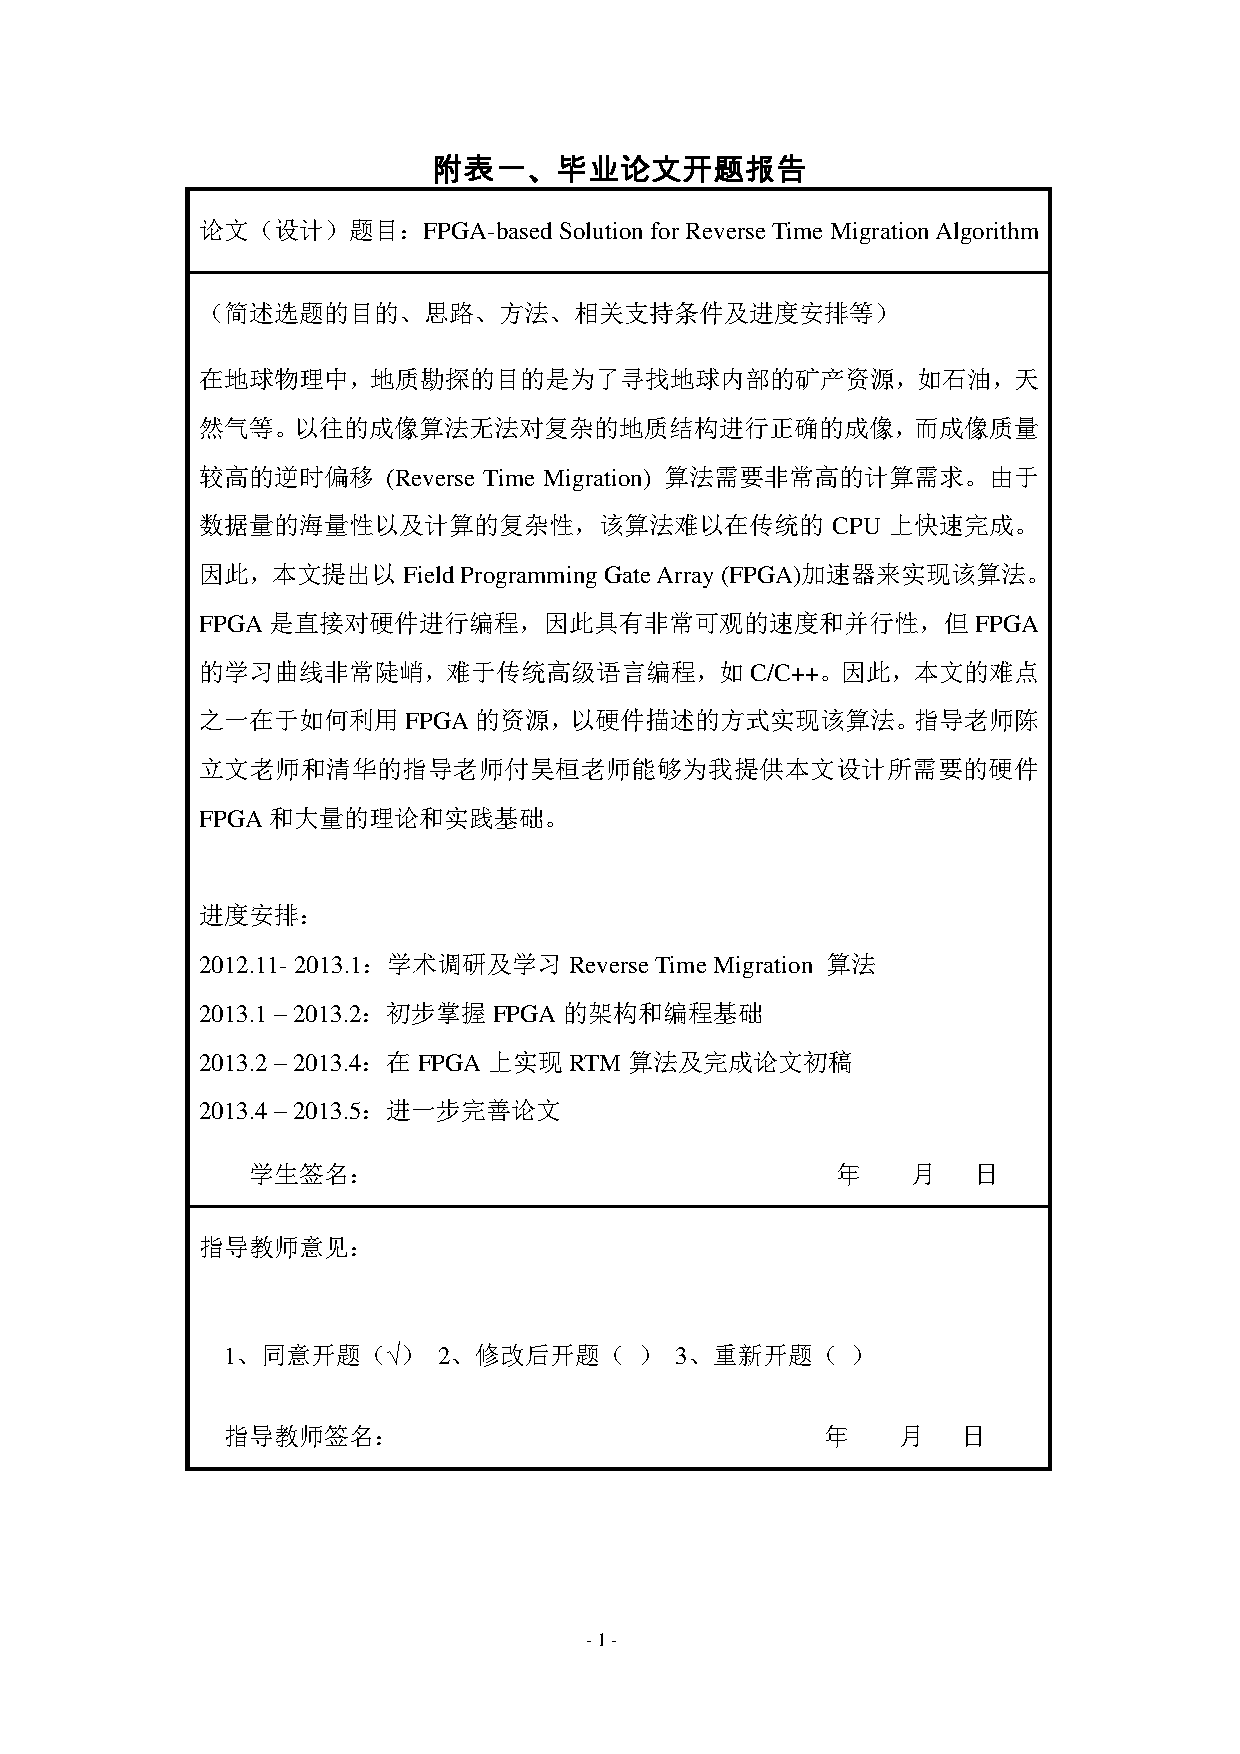
\includepdf{appendix/appendix1_proposal.pdf}
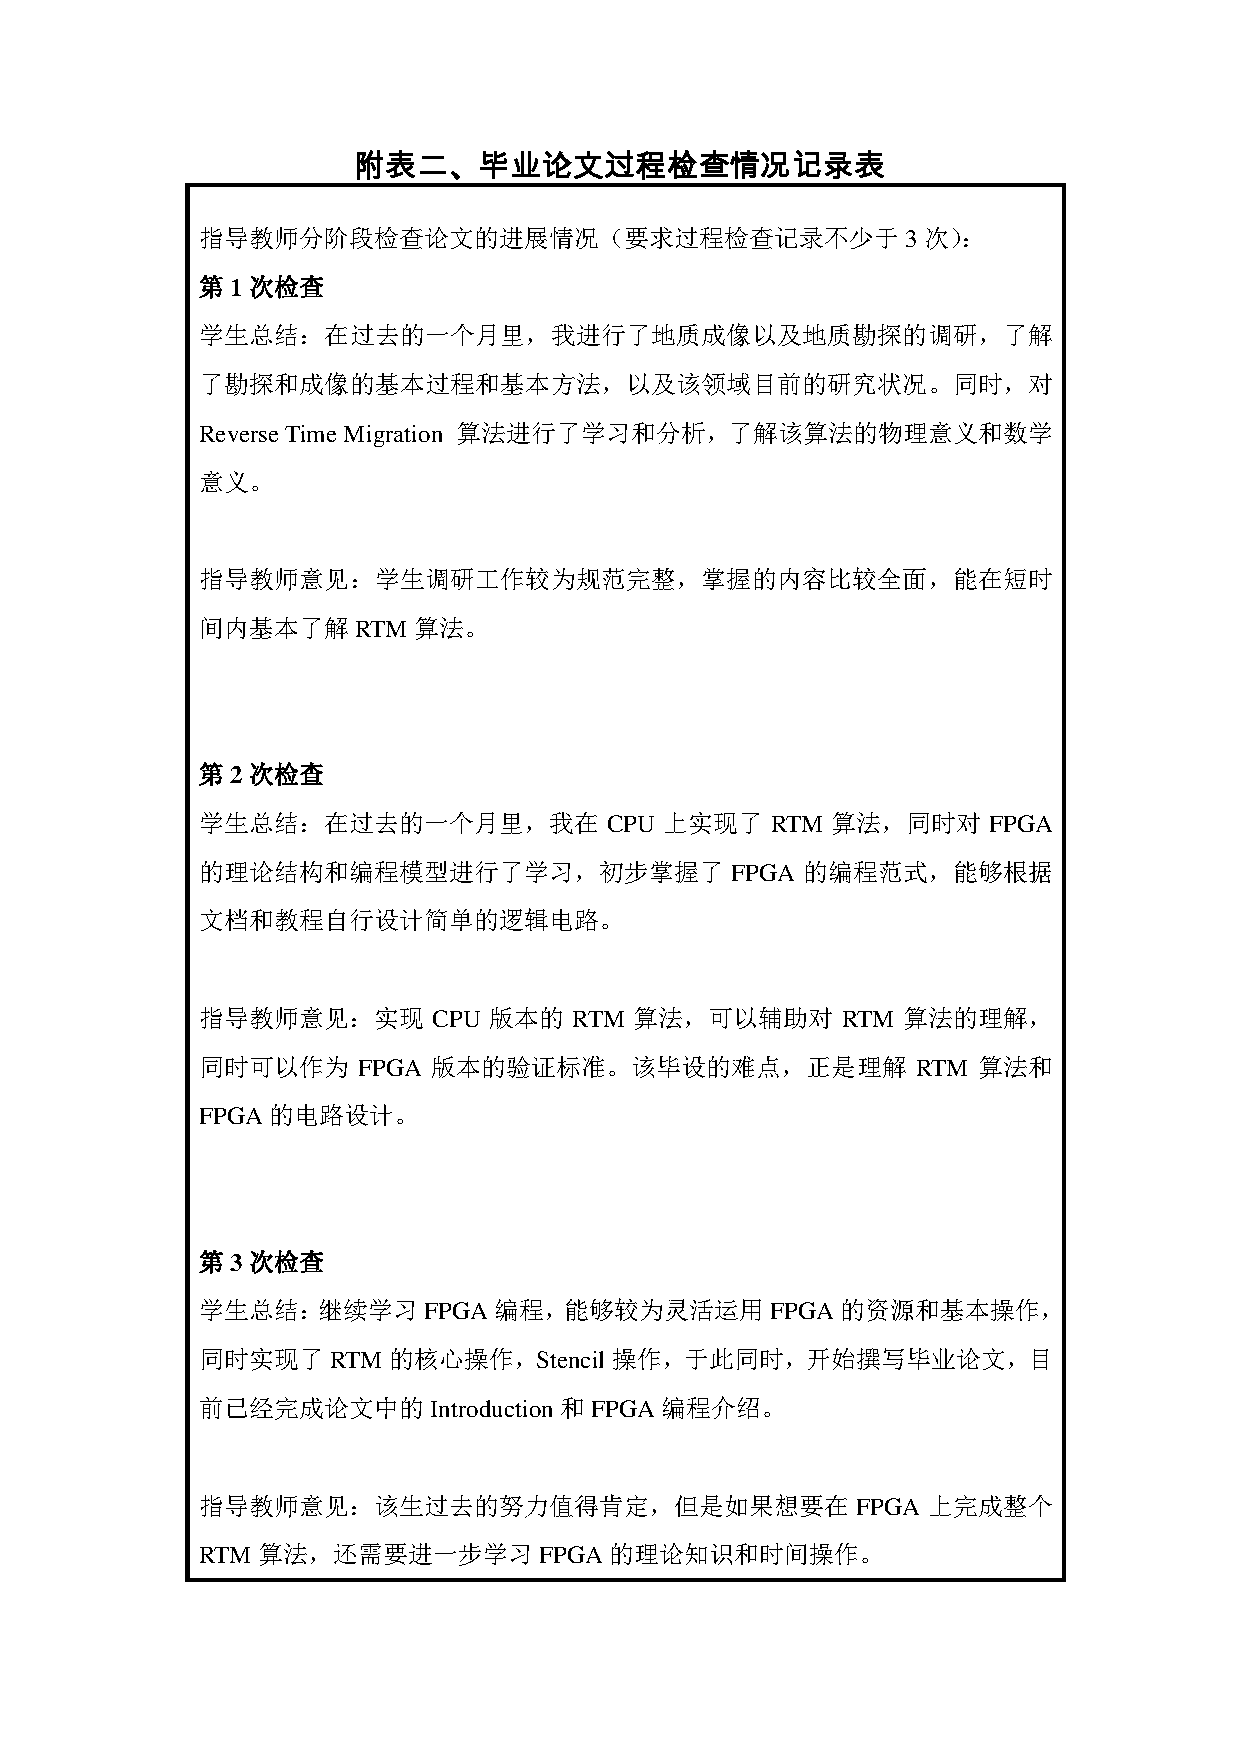
\includepdf{appendix/appendix2_records.pdf}
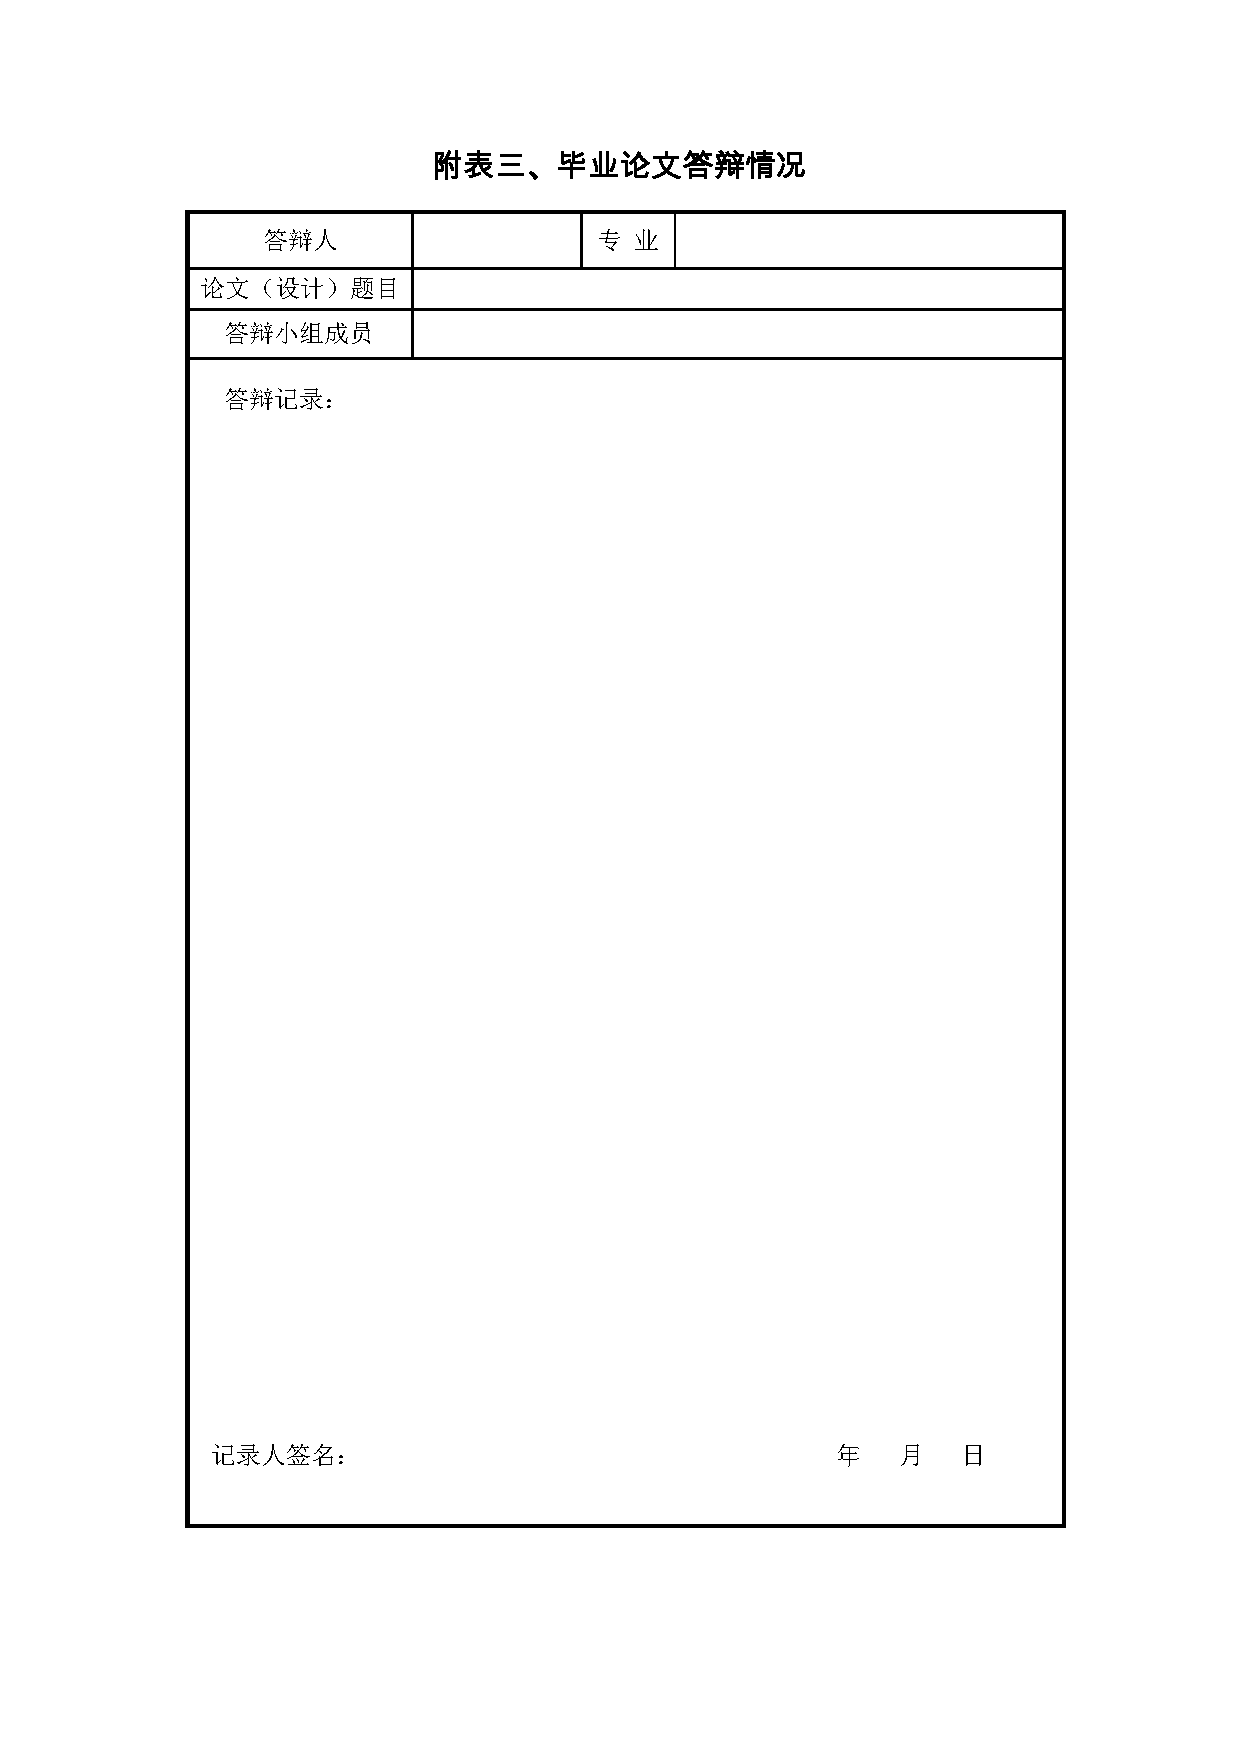
\includepdf{appendix/appendix3_scores.pdf}
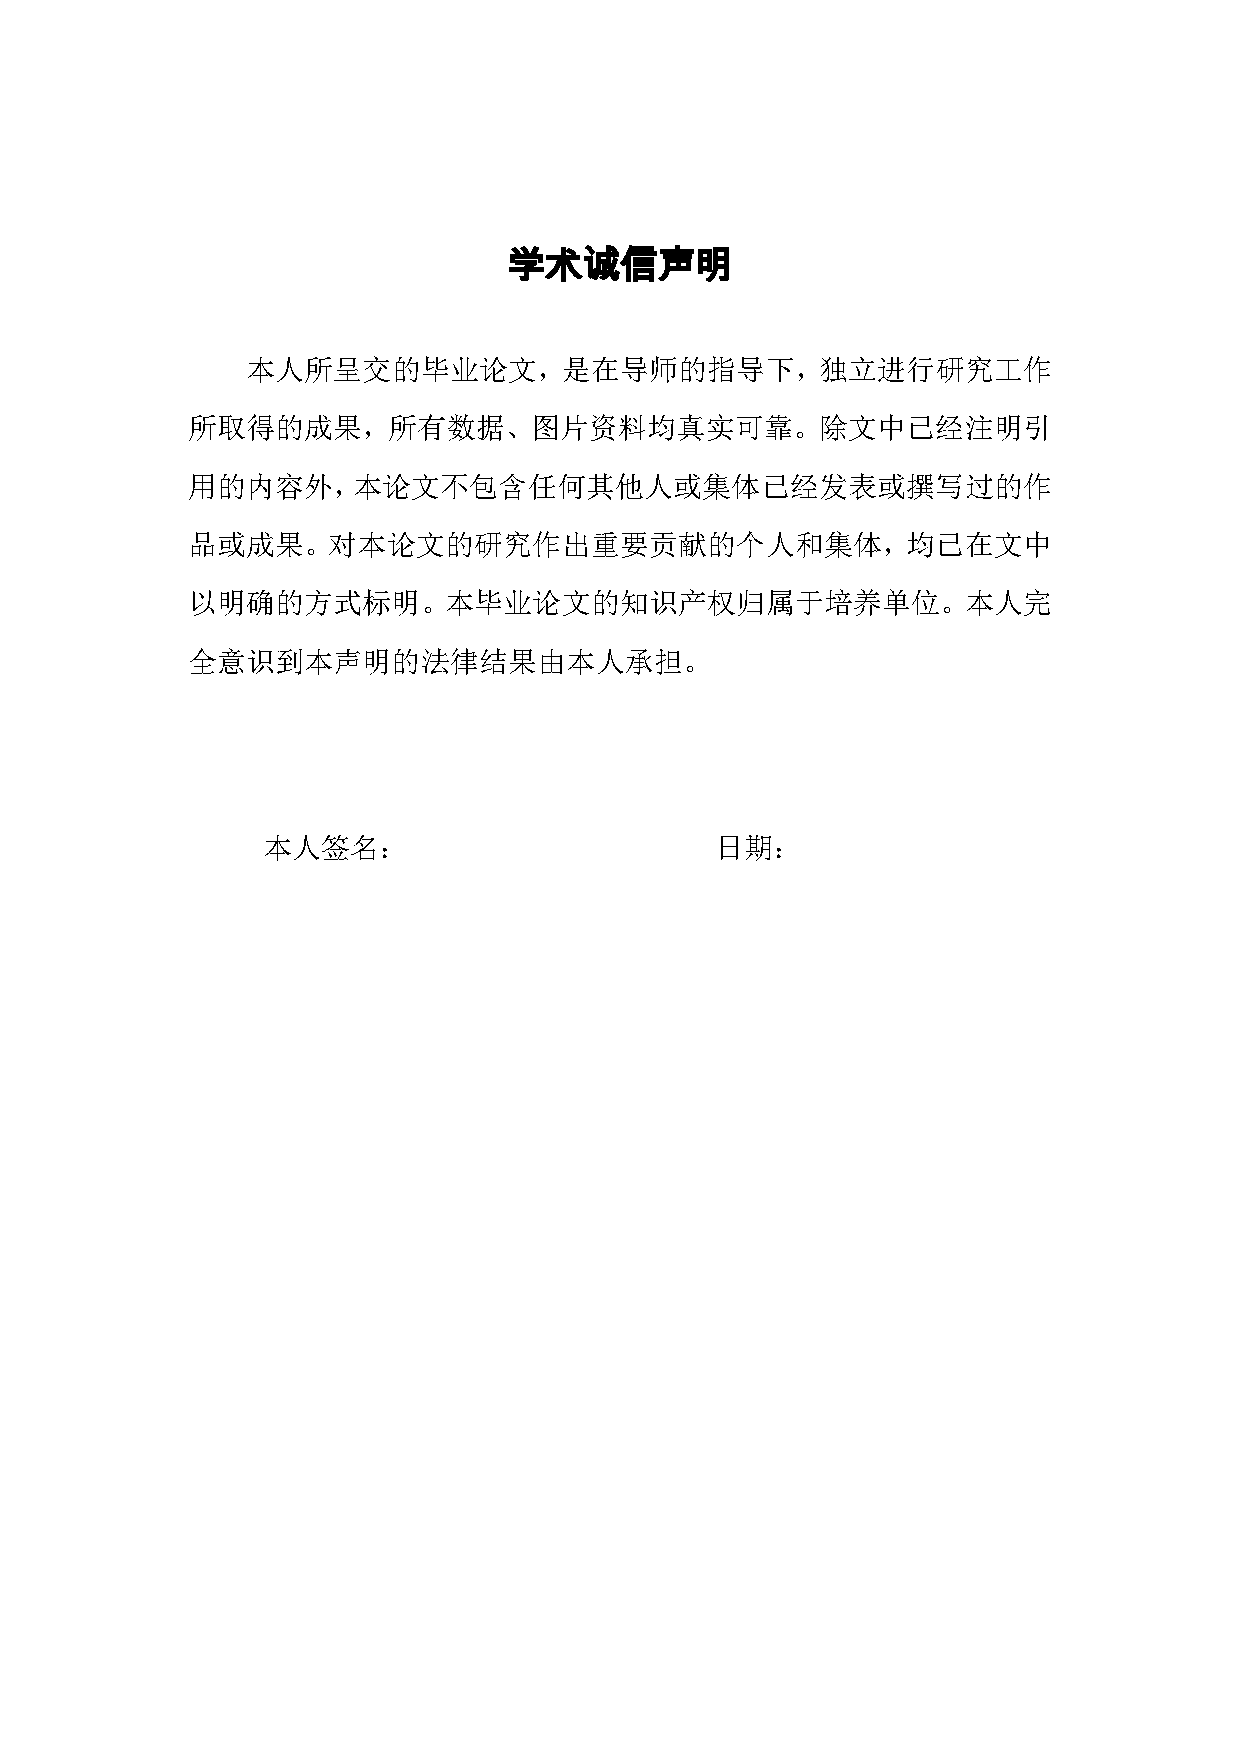
\includepdf{appendix/appendix4_honest_declaration.pdf}
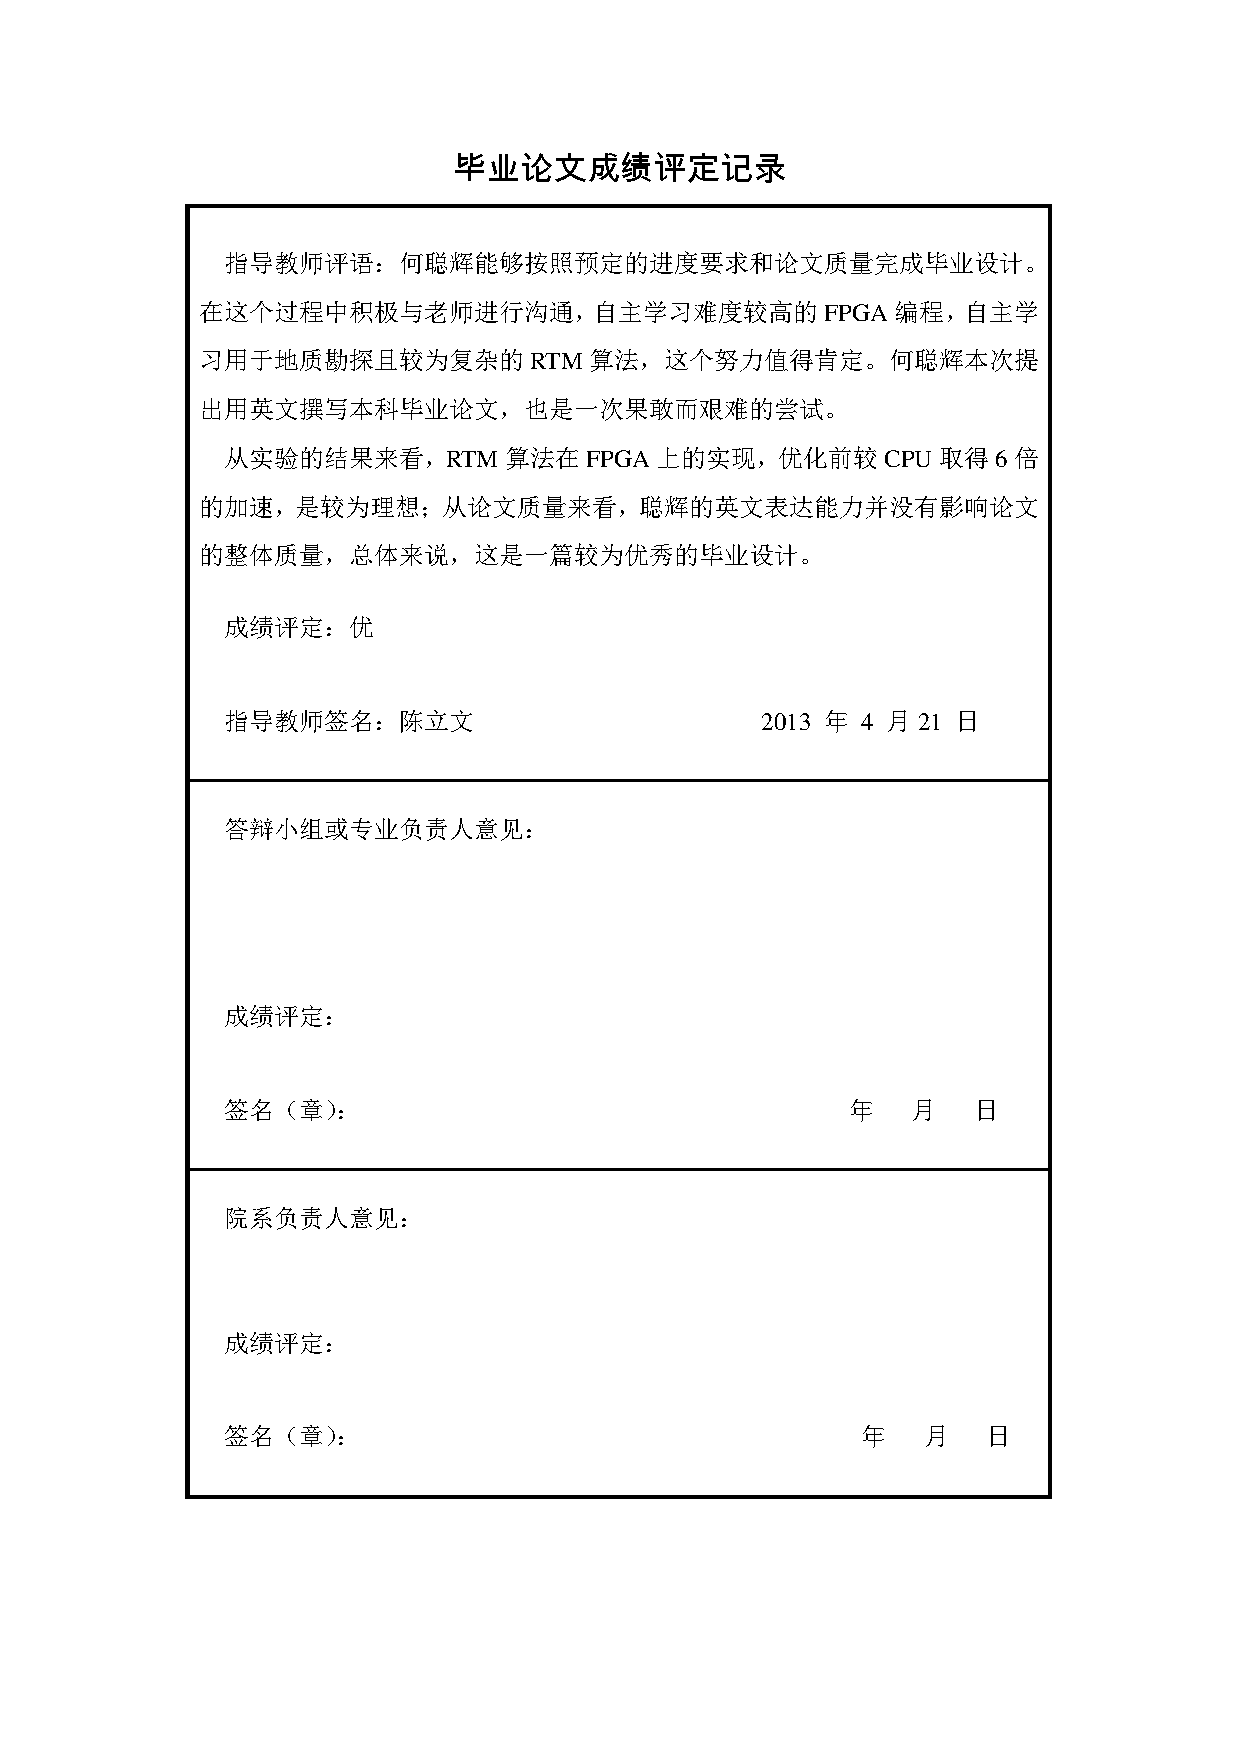
\includepdf{appendix/appendix5_evaluation.pdf}

\end{document}
